\documentclass[11pt,a4paper]{report}

\usepackage{url}
\usepackage[utf8]{inputenc}
\usepackage{graphicx}
\usepackage{array}
\usepackage{listings}
\usepackage{rutitlepage}
\usepackage[
backend=biber,
style=ieee,
sorting=nty,
maxcitenames=1,
mincitenames=1]{biblatex}
\addbibresource{bibliography.bib}
\usepackage[hidelinks]{hyperref}
\usepackage[inline]{enumitem}
\usepackage{caption}
\captionsetup[figure]{font=footnotesize,labelfont=footnotesize}
\captionsetup[table]{font=footnotesize,labelfont=footnotesize}
\captionsetup[lstlisting]{font=footnotesize,labelfont=footnotesize}
\usepackage[T1]{fontenc}
\usepackage{makecell}
\usepackage{multirow}

\makeatletter %otherwise geometry resets everything
\Gm@restore@org%
\makeatother

\setlength{\itemsep}{0cm}
\setlength{\voffset}{0cm}
\setlength{\headheight}{0cm}
\setlength{\topmargin}{0cm}
\setlength{\extrarowheight}{3pt} %for superscripts in tabular
\setlength{\arraycolsep}{4pt}
\lstset{basicstyle = \footnotesize, breaklines = true}

\graphicspath{{imgs/}}
\hyphenation{bench-mark-ing da-ta-base im-prov-ing trans-ac-tion in-di-vid-u-al-ly through-put in-tro-duc-tion bench-mark in-de-pend-ent-ly con-straints ex-per-i-men-tal per-for-mance meta-da-ta re-spec-tive-ly gen-er-al ver-sions trans-for-ma-tion in-ves-ti-gate tech-nol-o-gies spe-cif-ic ex-per-i-ments net-work rep-re-sen-ta-tion lake-house com-mu-ni-ca-tion min-i-mum in-for-ma-tion per-cent-age im-prove-ment through-out per-cent-ages op-er-a-tion sys-tems}

\begin{document}
\maketitleru[
    layout=traditional,
	authors={Vinícius Ribeiro Machado Schmidt\\s1123702},
	date={\today},
	others={%
        {University supervisor:}{prof.\ dr.\ ir.\ Djoerd Hiemstra \\ \nolinkurl{hiemstra@cs.ru.nl}},
        {Company supervisors:}{Chrystel Philipsen\\ \nolinkurl{chrystel.philipsen@sogeti.com}\\ Marcel de Wit \\ \nolinkurl{marcel.de.wit@sogeti.com}},
		{Second assessor:}{dr.\ Johannes Textor \\ \nolinkurl{johannes.textor@ru.nl}}
    },
	course={Master's Thesis Computing Science},
	title={\LARGE Evaluating Data Stream Write Performance in Lakehouse Systems},
    subtitle={}
]

\input{abstract}
\tableofcontents

\chapter{Introduction}\label{ch:introduction}

% Introduce the topic of the thesis, including research questions.

\section{Motivation and research questions}

% TODO: Give a bit of background on lakehouses, their design and the issues they aim to solve. Explain how each of the three lakehouses works and then transition into the research questions.

Many modern data storage architectures rely on so-called \textit{data lakes}, which consist of cloud object stores, e.g. Amazon S3\footnote{\url{https://aws.amazon.com/s3/}}, Azure Blob Storage\footnote{\url{https://azure.microsoft.com/en-us/products/storage/blobs/}}, for storing large amounts of (un)structured and semi-structured data in a centralized place \cite{WhatDataLake}. Part of the data can then be copied into data warehouses through a process called "extract, transform, load" (ETL), so that it can be used for further downstream analytics tasks \cite{michael_armbrust_lakehouse_2021}. Although this two-tier architecture has become widespread among many enterprises, it has a few drawbacks. ETL pipelines used to load data into warehouses can be time-consuming and error-prone, causing the data in the warehouse to be outdated and sometimes inconsistent \cite{schneider_lakehouse_2024}. Additionally, maintaining the two systems is expensive and redundant, since part of the data is stored in both the data lake and the warehouse \cite{michael_armbrust_lakehouse_2021}. Finally, the flexibility of storing various file formats in the same place comes with the cost of managing different file versions and metadata, which with time can transform the data lake into a "data swamp" \cite{avrilayshaDeltaLakeVs}.
 
Following the limitations of data lakes and the two-tier architecture, \citeauthor{michael_armbrust_lakehouse_2021} \cite{michael_armbrust_lakehouse_2021} proposed a new data storage architecture called \textit{data lakehouse}. A lakehouse, also referred to as an open table format, builds on top of data lakes by structuring data into tables that are stored in immutable columnar formats, e.g. Apache Parquet\footnote{\url{https://parquet.apache.org/}}. These tables are managed with centralized metadata files that keep track of the current schema and the different versions of the table, all while ensuring that updates to tables occur in ACID \cite{haerderPrinciplesTransactionorientedDatabase1983} transactions \cite{michael_armbrust_lakehouse_2021}. Furthermore, the use of open formats for storage gives users control over their data, in contrast to proprietary formats of data warehouses \cite{michael_armbrust_lakehouse_2021, schneider_lakehouse_2024, avrilayshaDeltaLakeVs}. These characteristics allow analytical tasks to be performed directly on the lakehouse tables, thus eliminating the need of having a separate data warehouse, thus eliminating the need for a two-tier architecture.

Although open table formats have gained popularity since their introduction, some aspects of lakehouses have led to important questions in recent works. For instance, \citeauthor{paras_jain_analyzing_2023} \cite{paras_jain_analyzing_2023} suggest that performing high frequent insertions into lakehouse tables can be challenging, because every insertion creates a new data file and requires updating the metadata files as well. Further, inserts in Delta Lake, a popular lakehouse format, can have up to hundreds of milliseconds of latency due to its reliance on object stores, which limits the throughput of streaming workloads, as mentioned in \cite{armbrust_delta_2020}. By contrast, the recent introduction of DuckLake \cite{mark_raasveldt_ducklake_2025} brought significant changes on how to handle write transactions to tables, while still ensuring ACID transactions. This is all thanks to the use of a traditional database management system (DBMS), e.g. PostgreSQL\footnote{\url{https://www.postgresql.org/}}, for handling table metadata. Interestingly, no work has been done yet to evaluate the throughput of open table formats when performing data stream insertions. Therefore, this thesis will fill that gap, by focusing on the following research question:

% Consequently, this raises the question of just how well-suited current lakehouse systems really are at meeting data stream processing (DSP) requirements. For example, the authors in \cite{paras_jain_analyzing_2023} conducted an evaluation of three different lakehouse systems on the TPC-DS benchmark \cite{TPCBENCHMARKDS2024} and suggested to further investigate the ability of lakehouses at handling workflows with a high number of concurrent write queries per second. They believe that this would be a challenging task for lakehouse systems due to the relatively high latency of communicating with the object store for updating the metadata on every write operation \cite{paras_jain_analyzing_2023}. Additionally, the authors in \cite{armbrust_delta_2020} mention that inserts in Delta can have up to hundreds of milliseconds of latency due to its reliance on object stores' implementations of put-if-absent operations for guaranteeing atomicity of transaction logs. Despite this, \citeauthor{armbrust_delta_2020} claim that Delta suffices in providing fast enough execution for all its applications \cite{armbrust_delta_2020}. Meanwhile, DuckLake's design might result in lower latency writes, since all the metadata is written to traditional DBMSs, which are more efficient at handling multiple concurrent transactions.

\begin{center}
    "\textit{How can we evaluate the throughput of data streams in lakehouse systems?}"
\end{center}

% Alternative
% \begin{center}
%     "\textit{How can we systematically evaluate streaming write performance in lakehouse systems?}"
% \end{center}

In addition, the following sub-questions will be answered 
\begin{enumerate}
    \item What are the current state-of-the-art benchmarks for lakehouses?
    % \begin{enumerate}
    %     \item What metrics are relevant for evaluating the performance of data streaming writes?
    % \end{enumerate}
    % \item What are the state-of-the-art datasets used for benchmarking streaming systems?
    \item What are common patterns used in benchmarks for stream processing systems?
    \item How can we ensure our benchmark is actually fair?
    \item What is the difference in performance of current lakehouse systems when evaluated with our benchmark?
    \begin{enumerate}
        \item What is the performance gain of the "data inlining" feature of DuckLake in comparison to other lakehouse formats?
    \end{enumerate}
\end{enumerate}

\section{Contributions}


\section{Thesis structure}
The rest of this thesis is structured as follows: Chapter \ref{ch:background} goes over the relevant background for this thesis, such as the different lakehouse technologies, how they are implemented and relevant features for this research. Chapter \ref{ch:related-work} talks about the existing work on benchmarking lakehouses and the different metrics employed by these benchmarks and the systems that they evaluate. Chapter \ref{ch:methodology} describes the methodology employed to develop our own benchmark and the reasoning behind those decisions. We also describe our experimental setup here. Chapter \ref{ch:results} present the results of our experiments, which will be discussed in Chapter \ref{ch:discussion}. Finally, Chapter \ref{ch:conclusion} will conclude this thesis by looking back at the proposed research questions, while proposing possible directions for future work.

\chapter{Background}\label{ch:background}

% TODO: Mention that lakehouses (or log structure table formats) are merely a specification and rely on specific implementations to be used, e.g. Spark's implementation of Delta and Iceberg, delta-rs and PyIceberg are all implementations of the spec. In this case, Spark is a query engine, while the other two are libraries that enable interaction with the tables through client APIs. This distinction is especially relevant when comparing the table formats, since it's not fair to compare the performance of a query engine with a client library. 

% TODO: Maybe mention what Parquet is and what the different compression options are, since they are the only relevant config that we will tune in our experiments.

Before we can develop our benchmark, we need to first understand how lakehouses work and which characteristics are relevant to the goal of this thesis. We will look at Iceberg and Delta Lake (Sections \ref{sec:lakehouse-iceberg} and \ref{sec:lakehouse-delta}), which are the two most popular and more mature lakehouse formats based on GitHub stars count and initial release date respectively \cite{thedeltalakeprojectauthorsDeltaLake2026, Iceberg2025}. Moreover, we will look at DuckLake, which brings innovative and relevant features for our research (discussed in Section \ref{sec:lakehouse-ducklake}), despite it still being in version 0.3.

This chapter will also go over the definitions of data stream and throughput, as well as guidelines on performing fair benchmarking.

% We will first go over the different lakehouse technologies included in this thesis: Apache Iceberg, Delta Lake and DuckLake. We will talk about their architectural design, how they handle reads and writes and how they deal with changing data. 

\section{Iceberg}\label{sec:lakehouse-iceberg}
Iceberg was developed in 2017 at Netflix and in 2018 it was released as an open-source project within the Apache Software Foundation\footnote{\url{https://www.apache.org/}}.

\subsection{Architectural design}

\begin{figure}
    \centering
    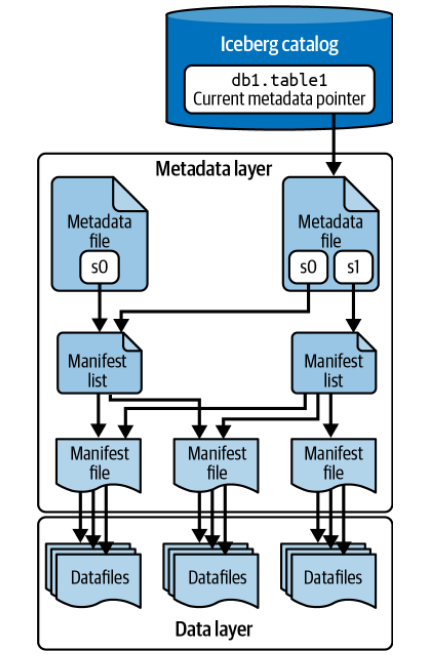
\includegraphics[width=0.45\linewidth]{imgs/iceberg-architecture.png}
    \caption{Architecture of an Iceberg table, as presented in \cite{jasonhughesApacheIcebergDefinitive2024}.}
    \label{fig:iceberg-architecture}
\end{figure}

\subsubsection{Data layer}
 At the base of Iceberg's architecture, there is a data layer, which consists of data files that constitute the Iceberg table. They can be stored in one of three formats: Parquet, ORC\footnote{\url{https://orc.apache.org/}} or Avro\footnote{\url{https://avro.apache.org/}}, with Parquet being the most common due to its widespread adoption and performance gains \cite{jasonhughesApacheIcebergDefinitive2024}.

% The delete files use the same file format as data files, but, as the name suggests, they are a exclusively used for tracking rows that have been deleted from the Iceberg table. There are three different types of delete files in Iceberg, namely:

% \begin{itemize}
%     \item \textbf{Equality delete files}: These files track specific column values that match one or more rows to be deleted from a table \cite{jasonhughesApacheIcebergDefinitive2024}. For instance, if a table contains users' actions on a website, one could delete all actions associated with a user by creating an equality delete file that references that user's id.
    
%     \item \textbf{Positional delete files}: These files keep track of rows to be deleted by storing the path to a data file and the row numbers in that file \cite{jasonhughesApacheIcebergDefinitive2024}. Positional delete files have been deprecated in Iceberg table spec V3 in favor of deletion vectors \cite{apacheicebergIcebergTableSpec}.
    
%     \item \textbf{Deletion vectors}: Introduced in Iceberg table spec V3, deletion vectors replace positional delete files by keeping track of deleted rows of a data file in a bitmap \cite{apacheicebergIcebergTableSpec}. Each vector is associated with one data file, where each bit of the bitmap has the same position as its corresponding row in the data file.
% \end{itemize}

\subsubsection{Metadata layer}\label{sec:iceberg-metadata}

Besides the data layer, there is the metadata layer, which keeps track of the data files locations, the version history of the table, as well as its current schema. The files in the metadata layer are:

\begin{itemize}
    \item \textbf{Manifest files}: Stored in Avro format, these files store pointers to multiple data files, as well as metadata about them, such as the minimum and maximum values of a file's columns and the number of records \cite{jasonhughesApacheIcebergDefinitive2024}. The metadata in manifest files is used for filtering data files during read operations, which helps improve read performance \cite{jasonhughesApacheIcebergDefinitive2024}.

    \item \textbf{Manifest lists}: Manifest lists are another set of Avro files that individually point to a collection of manifest files. Together, the manifest files referenced by a manifest list constitute a specific snapshot, i.e. version, of an Iceberg table \cite{jasonhughesApacheIcebergDefinitive2024}.

    \item \textbf{Metadata files}: These are JSON files that contain schema information about the table, as well as the snapshot history and a pointer to the current snapshot of that table \cite{jasonhughesApacheIcebergDefinitive2024}. A new metadata file is created after every update to the table, marking the creation of a new snapshot. Figure \ref{fig:iceberg-architecture} depicts the architecture of an Iceberg table, where the newest metadata file has a pointer to both snapshots "s0" and "s1".
\end{itemize}

\subsubsection{Catalog}
In order to manage Iceberg tables, a catalog server is used. The goal of the catalog is to point to the latest metadata file of a table, as well as ensure that this pointer is updated atomically \cite{IcebergSpecOptimistic, jasonhughesApacheIcebergDefinitive2024}. Consequently, all interactions with an Iceberg table must go through the catalog server. This avoids inconsistencies when clients are concurrently writing to the same table.

Although many technologies can be used as catalog, e.g. AWS Glue\footnote{\url{https://docs.aws.amazon.com/glue/latest/dg/what-is-glue.html}} and Hive Metastore\footnote{\url{https://hive.apache.org/}}, the developers of Iceberg provide a REST API spec \cite{apacheicebergRESTCatalogSpec2025} as an attempt to unify catalog access across different engines and languages. One prominent implementation of the Iceberg REST catalog is Apache Polaris\footnote{\url{https://polaris.apache.org/}}, which uses a PostgreSQL database to store the latest metadata pointer. 

% \subsection{Reading from Iceberg tables}
% Reading data from Iceberg can be broken down into five steps, as described in \cite{jasonhughesApacheIcebergDefinitive2024}:
% \begin{enumerate}
%     \item The query engine retrieves the pointer to the latest metadata file.
    
%     \item The engine then reads the current table schema and partitioning information, as well as the path to the manifest list.

%     \item From the manifest list, the engine reads the path to the manifest files.

%     \item In each manifest file, the engine checks the data files it points to, possibly skipping over data file partitions that are not included in the query. In addition, the query also checks statistics such as min and max values of columns in the data files, so that it can skip individual data files.

%     \item Once the relevant data files have been selected, the query engine then reads them and returns the result
% \end{enumerate}

\subsection{Writing to Iceberg tables}\label{sec:iceberg-writing}
Writing data to an Iceberg table, e.g. via \verb|INSERT|, involves the following steps \cite{jasonhughesApacheIcebergDefinitive2024}:
\begin{enumerate}
    \item First, the engine checks the catalog to get a pointer to the current metadata file, so that it can read the current table schema.

    \item New data file(s) are written using the chosen storage format for the table.

    \item The engine will then write the manifest file(s) that will contain metadata about the new data file(s), as well as a pointer to them.

    \item Next, a new manifest list file is created, which will point to the new manifest file(s). In addition, existing manifest files are added to this new list, which together will correspond to the new snapshot of the table.

    \item The engine writes a new metadata file which contains a pointer to the new snapshot (manifest list), as well as a history of all previous snapshots.

    \item Finally, following the principle of optimistic concurrency \cite{IcebergSpecOptimistic}, the engine will assume the table has not changed since the start of the operation and will try to atomically update the catalog to point to the new metadata file. However, if a concurrent write has created a new snapshot in the meantime, changing the metadata pointer fails and the engine has to retry. Iceberg tries to structure changes in such a way to minimize the cost of retries \cite{apacheicebergReliability}.
\end{enumerate}

\section{Delta Lake}\label{sec:lakehouse-delta}

Delta Lake was introduced in \citeyear{armbrust_delta_2020} by \citeauthor{armbrust_delta_2020} \cite{armbrust_delta_2020}. It was originally developed at Databricks\footnote{\url{https://www.databricks.com/}} and it was open-sourced in 2022 \cite{tathagatadasDelta20Foundation2022}.

\subsection{Architectural design}

\begin{figure}[h!]
    \centering
    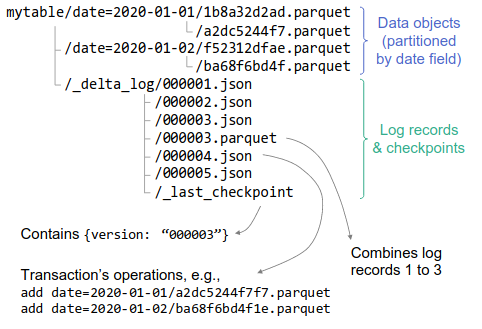
\includegraphics[width=0.6\linewidth]{imgs/delta-architecture.png}
    \caption{The architecture of a Delta Lake table, as presented in \cite{armbrust_delta_2020}.}
    \label{fig:delta-architecture}
\end{figure}

\subsubsection{Data files}

At its core, a Delta table consists of a directory containing data files, which are stored in the Parquet format. As shown if Figure \ref{fig:delta-architecture}, this data can be partitioned to improve efficiency of read queries, but this is beyond the scope of this thesis.

% In addition, Delta stores deletion vectors at the root of a table directory \cite{lee_delta_2025}, which are binary files that keep track of deleted rows of a table. It does so by tracking the offset of a row in the file, its size and the number of rows (cardinality) that has been deleted \cite{lee_delta_2025}.

\subsubsection{Delta log}

The metadata of a Delta table is stored in a subdirectory, called "delta log". This directory contains JSON files, each named in increasing order according to the table version they correspond to, e.g. \verb|00001.json|, \verb|00002.json|, \verb|00003.json|, etc. The log files themselves consist of actions, e.g. \verb|add| and \verb|remove|, that were applied to the data files in order to obtain the respective version \cite{armbrust_delta_2020}.

Furthermore, Delta also keeps track of so-called "checkpoint" files. These are Parquet files consisting of all the actions in the JSON files up until that point in time. These checkpoint files are created periodically (the default being every 10 transactions), so that Delta can stay performant when reconstructing the current state of a table from the log files \cite{armbrust_delta_2020}. The name of the most recent checkpoint file is stored in a \verb|_last_checkpoint| file, as depicted in Figure \ref{fig:delta-architecture}.

\subsubsection{Catalog}

\begin{figure}
    \centering
    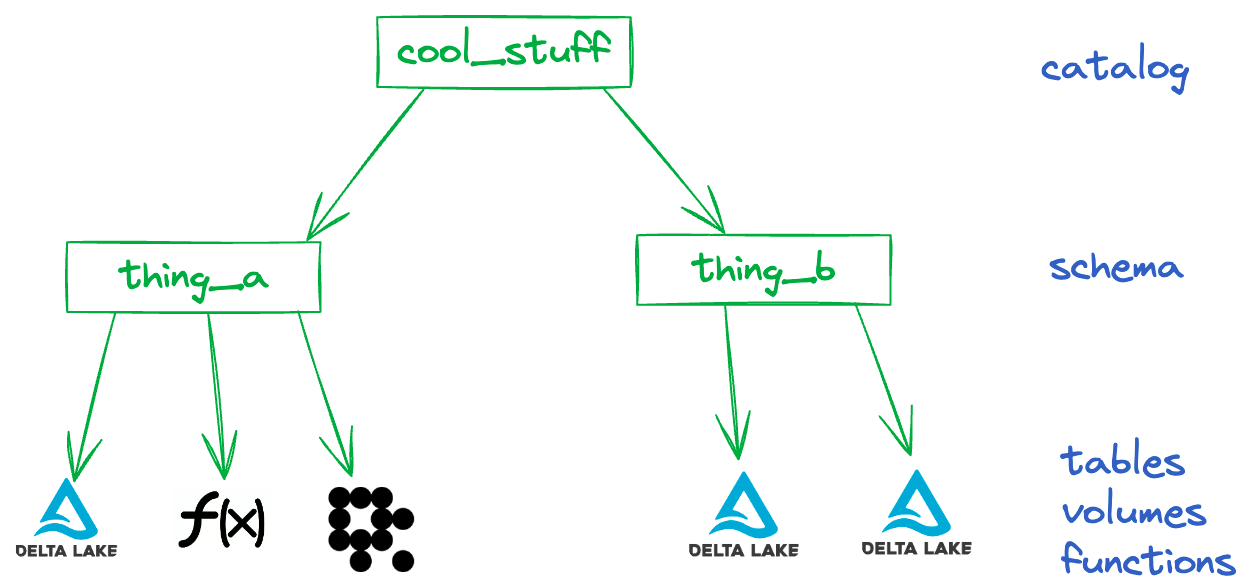
\includegraphics[width=0.8\linewidth]{imgs/unity-catalog.png}
    \caption{Overview of a Unity Catalog, which can be used to manage multiple Delta Lake tables \cite{UnityCatalogStructure2024}.}
    \label{fig:unity-catalog}
\end{figure}

Delta Lake can be connected with a catalog, allowing the management of multiple tables and creating interoperability between other open table formats, such as Iceberg. The most popular catalog used to manage Delta tables is Unity Catalog\footnote{\url{https://www.unitycatalog.io/}}. There are two versions of this catalog: A proprietary version maintained by Databricks and an open-source version. We focus on the latter, since it is freely available. Similar to the Polaris catalog, the Unity Catalog server can be accessed through a REST API and it uses a relational database to store information about the Delta tables that it knows about.

Although a catalog server is not part of the Delta Lake specification, as it is in Iceberg's case, we include it in our research to make sure we perform a fair comparison between the systems we are analyzing (see also Section \ref{sec:benchmarking}).

% \subsection{Reading from Delta tables}
% Below we describe the steps taken by the Delta engine when reading a table \cite{armbrust_delta_2020}:

% \begin{enumerate}
%     \item Delta will first look for the \verb|_last_checkpoint| file. Using the checkpoint file's ID, all subsequent log and checkpoint files are listed.

%     \item Using the listed files, the engine will read them to reconstruct the current state of the table, as well as statistics such as min and max values of columns and partitioning information.

%     \item Based on the table statistics, the engine can ignore files that are irrelevant to the query, which helps improve performance.

%     \item Finally, the relevant data files are queried and the result is returned. 
% \end{enumerate}

\subsection{Writing to Delta tables}
The process of writing data to a Delta table can be broken down into the following steps \cite{armbrust_delta_2020}:

\begin{enumerate}
    \item Delta will first look for the \verb|_last_checkpoint| file. Using the checkpoint file's ID, all subsequent log and checkpoint files are listed.

    \item Using the listed files, the engine will read them to reconstruct the current state of the table, as well as statistics such as min and max values of columns and partitioning information.

    \item Once all those files have been read, new data objects are written (possibly in parallel) to the underlying file storage.

    \item Then, assuming the latest log file has ID $n$, Delta attempts to create a new log file named $n+1$\verb|.json|. Since there can only be one file corresponding to a specific version of the table, creating the new log file needs to happen atomically. If this step fails due to a concurrent write operation, the transaction can be retried.

    \item (Optional) Depending on the configured interval for writing checkpoints, a new checkpoint file will be created and the \verb|_last_checkpoint| file is updated to reflect that change.
\end{enumerate}

It is important to note that, like in Iceberg (Section \ref{sec:iceberg-writing}), optimistic concurrency control is employed for write operations. However, Delta relies on the underlying object store's mechanism to ensure transaction atomicity \cite{armbrust_delta_2020}. For instance, Azure Blob Store, Google Cloud Storage and Amazon S3 support conditional write operations \cite{SpecifyingConditionalHeaders2025, RequestPreconditions2026, HowPreventObject}, thus ensuring that only one client can create a log file with a specific name.

% So if a new log file ($n+1$\verb|.json| in this case) is created between the start and end of a write operation, that operation fails and needs to retry. Again, as it is the case for Iceberg, there are optimizations in place that allow the engine to retry the operation without having to rewrite all files, depending on the query \cite{armbrust_delta_2020}. In any case, this can lead to overhead when concurrent writes are happening in Delta Lake.

\section{DuckLake}\label{sec:lakehouse-ducklake}
DuckLake is an open table format introduced in 2025 as part of the DuckDB Foundation. Although it is currently an experimental release (as of writing, the current version is 0.3 \cite{guillermosanchezDuckLake03Iceberg2025}), we believe it will be a valuable addition to our research, as its specification proposes a new way of storing metadata and an interesting approach for handling changes to its tables.

\subsection{Architectural design}

\begin{figure}
    \centering
    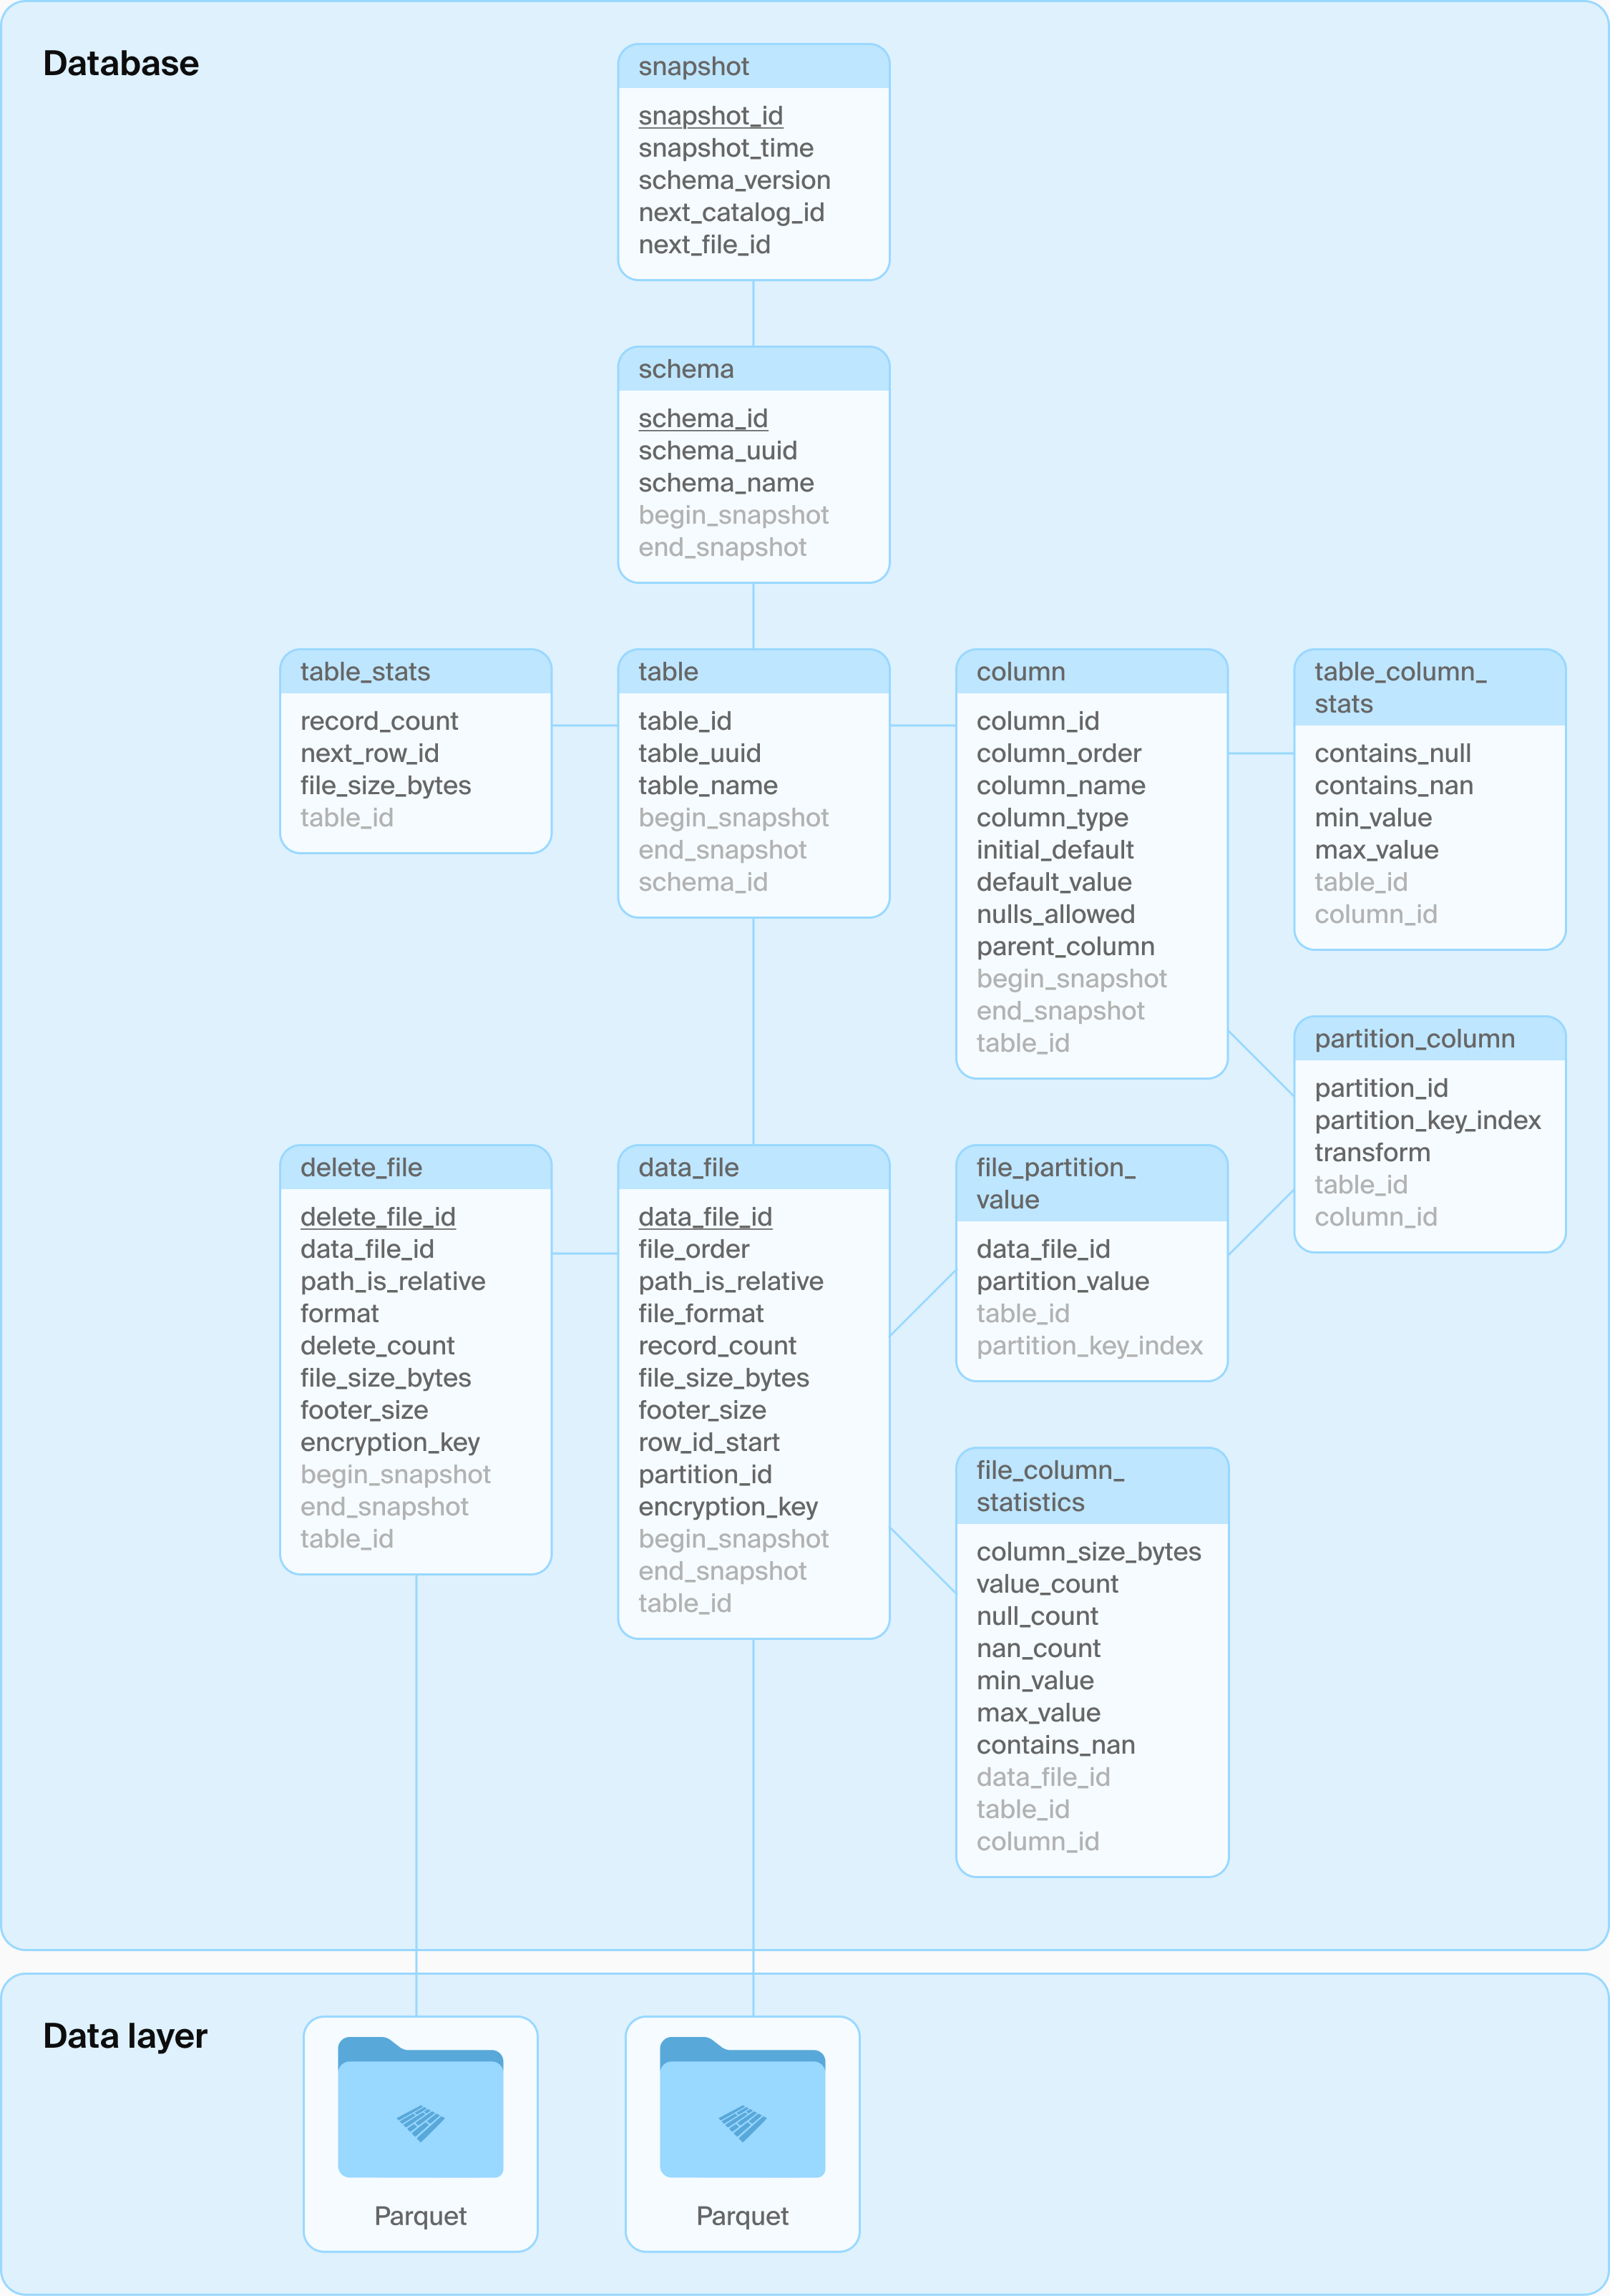
\includegraphics[width=\linewidth]{imgs/ducklake-architecture.png}
    \caption{Architecture of a DuckLake table, as presented in \cite{mark_raasveldt_ducklake_2025}.}
    \label{fig:ducklake-architecture}
\end{figure}

\subsubsection{Data layer}
DuckLake's data layer consists of Parquet data files on the chosen storage system, which make up the table.

\subsubsection{Catalog database}
Similar to Iceberg, DuckLake also includes a catalog in its specification. However, DuckLake's catalog differs from Iceberg's in that it stores all of the table's metadata instead of storing the pointer to the current metadata file. In total, the catalog database contains 22 tables that together keep track of the schema, snapshots, data files, tables, statistics and partitioning information of DuckLake tables \cite{DucklakeDocumentationTables2025}. Currently, DuckLake supports DuckDB\footnote{\url{https://duckdb.org/}}, SQLite\footnote{\url{https://sqlite.org/index.html}}, PostgreSQL and MySQL\footnote{\url{https://www.mysql.com/}} as its catalog database \cite{DucklakeDocumentationChoosing2025}. Figure \ref{fig:ducklake-architecture} shows the most relevant tables stored in the catalog \cite{DucklakeDocumentationTables2025}:

\begin{itemize}
    \item \verb|table|: This is where the DuckLake tables' name, path and schema are stored. In addition, it tracks the snapshot interval in which the table is valid.
    
    \item \verb|table_stats|: This contains metadata about the DuckLake tables, such as the number of records and the total file size of the data files that compose this table.
    
    \item \verb|column|: This table stores the columns that are part of the DuckLake table. The main attributes are the column's name, its type and default value.
    
    \item \verb|table_column_stats|: Similar to \verb|table_stats|, this table contains metadata about each column in a DuckLake table, e.g. min and max values and whether the column has \verb|NULL| values.
    
    \item \verb|partition_column|: Contains partitioning information about columns on which partitioning has been enabled. It also stores the transformation function that is applied to the column to obtain the partition key, if such a function is required. For instance, if a table contains a timestamp column, one can apply a transformation function to that column and use the resulting value as the partitioning key.    
    
    \item \verb|data_file|: This table stores information about the data files, such as the path, format (for now, only Parquet is allowed \cite{DucklakeDocumentationTables2025}), number of records in the file and the size in bytes.

    \item \verb|file_column_stats|: Similar to \verb|table_column_stats|, this table stores column statistics on a file level, e.g. amount of records, min and max values and number of \verb|NULL| values.

    \item \verb|delete_file|: Similar to \verb|data_file|, this table stores the path and format of delete files\footnote{Delete files are used to mark which records have been deleted from a table without actually deleting any files. This is done because Parquet files are immutable and would have to be rewritten every time a record is updated or deleted. By using delete files, deleted records can be reconciled at read time in a process called merge-on-read (MoW) \cite{paras_jain_analyzing_2023}, which is beyond the scope of this thesis.}, but it contains the number of records deleted by the file.

    \item \verb*|snapshot|: This table is used for representing the snapshots, i.e. versions, of the DuckLake instance. Every change to a table will result in a new snapshot with a corresponding timestamp.

    \item \verb|snapshot_changes|: For each snapshot, this table stores a list of changes that were made to the DuckLake instance, e.g. \verb*|CREATE|, \verb*|INSERT|, \verb*|UPDATE|, \verb*|ALTER|.

    \item \verb|schema|: This table stores the different schemas that can be used to separate DuckLake tables into namespaces. The table stores the schema name, its path in the file system, as well as the snapshot interval in which that schema is valid.
\end{itemize}

%\subsection{Reading from DuckLake tables}
%Reading from a DuckLake table goes as follows \cite{DuckLakeDocumentation2025}:
%
%\begin{enumerate}
%    \item DuckLake first reads the latest snapshot number from the \verb|ducklake_snapshot| table.
%
%    \item Then, it reads the valid schemas in the current snapshot from \verb|ducklake_schema|. By default all tables are stored under the \verb|main| schema.
%
%    \item Next, DuckLake lists the tables in the given schema.
%
%    \item For the tables, it lists all the columns to determine the table structure.
%
%    \item Knowing the table structure, DuckLake queries the data files and delete files, so that it can know which rows to display and which ones have been deleted.
%\end{enumerate}

\subsection{Writing to DuckLake}
Writing to DuckLake tables happens in the following steps \cite{mark_raasveldt_ducklake_2025}:

\begin{enumerate}
    \item First, the Parquet files are written to storage, unless data inlining (\ref{sec:ducklake-inlining}) is enabled and the number of inserted rows is lower than the set threshold.

    \item Then, in a single database transaction, the following tables are updated to reflect the new changes: 
    \begin{itemize}
        \item \verb|data_file|
        \item \verb|table_stats|
        \item \verb|table_column_stats|
        \item \verb|file_column_statistics|
        \item \verb|snapshot|
        \item \verb|snapshot_changes|
    \end{itemize}
    DuckLake enforces a primary key constraint on the snapshot id in the \verb|snapshot| table \cite{DuckLakeDocumentationConflict2025}. If two clients try to concurrently create a new snapshot, one of them will fail due to a \verb*|PRIMARY| \verb*|KEY| constraint violation \cite{DuckLakeDocumentationConflict2025}. In that case, DuckLake will try to solve the conflict without having to rewrite the data files. For that, it looks at the \verb|snapshot_changes| table to see what changes were made by the transaction that succeeded. If there are no logical conflicts, e.g. both clients just added new data, the failed client can retry the transaction without having to rewrite the data files \cite{DuckLakeDocumentationConflict2025}.
\end{enumerate}

\subsection{Data inlining}\label{sec:ducklake-inlining}
One feature that sets DuckLake apart from Delta and Iceberg is the so-called "data inlining". This feature allows DuckLake to be configured such that writes that insert fewer rows than a set threshold are stored in the catalog database, rather than written out as Parquet files \cite{DuckLakeDocumentationData2025}. This can increase the performance of DuckLake for frequent, small, updates. The "inlined" data is immediately visible for read operations and it can be flushed out to Parquet files once enough data has been accumulated in the catalog \cite{DuckLakeDocumentationData2025}.

% TODO: Probably remove this section, since we're not doing any updates.
%\section{Data update strategies}
%
%\subsection{Copy-on-write (CoW)}
%This update strategy is supported by both Delta and Iceberg and, as the name suggests, it consists of rewriting the data files when a table is updated or data is deleted to reflect those changes. This results in higher write latency in favor of faster reads \cite{paras_jain_analyzing_2023}.
%
%The main reason CoW exists is because file formats used for data files, e.g. Parquet, are immutable \cite{matthewpowersDeltaLakeVs}, which means that changing a single value in them requires a complete rewrite of the file. In addition, lakehouses make use of snapshots to provide "time traveling" features, which is only possible by storing the older version of data files in the lakehouse storage layer.
%
%\subsection{Merge-on-read (MoR)}
%By using deletion vectors, or other delete file types in the case of Iceberg and DuckLake, (see Sections \ref{sec:lakehouse-iceberg} and \ref{sec:lakehouse-delta}), it is possible to adopt a merge-on-read (MoR) strategy instead of CoW. In this case, no data files are rewritten during updates and deletes, but rather the affected rows are stored in deletion files, usually in binary format, which are then used to filter out the corresponding data from the table during read operations. This strategy favors faster writes, but adds extra overhead when reading a table, since the engine needs to resolve the deleted rows of each table by reading the delete files. 
%
%It is worth mentioning that the table size and the number of updated/deleted rows are of great influence to the effectiveness of delete files and MoR. For instance, if the table consists of only a few data files and the amount of affected rows comprises a high percentage of the table, the time difference between writing a deletion file and rewriting the data files might be negligible, in which case rewriting the table would be preferable (CoW), since there would be no additional overhead when reading the table later. However, if the table is partitioned into multiple data files, changes to rows could lead to rewriting many files, in which case deletion files would be beneficial.
%
%In order to keep lakehouses performant when using MoR, it is recommended to perform regular maintenance operations, which rewrite data files with a high number of deleted rows into fewer, or even a single, data file(s) \cite{DuckLakeDocumentation2025, nickkarpovDeltaLakeDeletion2023, apacheicebergMaintenance}.

% \section{Stream processing}
% Streaming data can be defined as data that is produced by one or more sources continuously and thus, is considered unbounded \cite{tylerakidauStreaming101World2015, fragkoulisSurveyEvolutionStream2024}. As opposed to finite datasets that can be processed in their entirety by methods such as MapReduce \cite{jeffreydeanMapReduceSimplifiedData2004}, streaming datasets usually do not have a "final" data point, so streaming processing engines (SPEs) rely on approaches such as (micro-)batching and windowing to create finite groupings from the unbounded data for processing \cite{tylerakidauStreaming101World2015}. Some use cases where stream processing is commonly applied, include IoT sensor-monitoring, fraud detection, advertisement analytics and processing of logs for web services \cite{yueSurveyStreamProcessing2026}.

% In the following sections, we will lay out the core concepts of streaming data processing that we will be referring to throughout this thesis. 

% \subsection{Event time}
% One of the core concepts of data stream processing is "event time", which refers to the timestamp when a given event was produced by a source \cite{tylerakidauStreaming101World2015, yueSurveyStreamProcessing2026}, e.g. an IoT sensor. Event time is primarily used for windowing events, which we will discuss later on.

% \subsection{Processing time}
% As the name implies, processing time refers to the moment when an event is processed by a streaming system. This is not necessarily equal to the time when an event enters the streaming system, sometimes referred to as "ingestion time" \cite{yueSurveyStreamProcessing2026}, but rather the time when the event is sent for downstream processing \cite{tylerakidauStreaming101World2015}, usually after a fixed time period.

% \subsection{Processing patterns}
% When it comes to actually processing the data, there are different techniques that SPEs apply to process unbounded streams of data in some type of bounded way.

% \subsubsection{(Micro) Batching}
% % Spark operates in this mode by default, with a default interval of 500ms (source: https://docs.databricks.com/aws/en/structured-streaming/triggers)
% The first way of processing streaming data is by grouping incoming data in batches that are processed at fixed time intervals. Since the interval is fixed, micro-batching relies solely on the processing time to create the micro batches. These intervals are usually kept at low values, e.g. Spark\footnote{\url{https://spark.apache.org/docs/latest/streaming/index.html}} uses intervals of 500ms by default \cite{ConfigureStructuredStreaming2023}, so that latency is kept at a low rate.

% \subsubsection{Windowing}
% Windowing is a more flexible technique for processing data streams, as it allows grouping events by both processing and event time \cite{tylerakidauStreaming101World2015}. There are three main types of windowing techniques, namely:

% \paragraph{Fixed windows}
% Also referred to as "tumbling window", this method groups events in non-overlapping fixed-length windows, which are then sent for downstream processing. When creating windows by processing time, this method works essentially the same way as micro-batching.

% \paragraph{Sliding windows}
% These windows also consist of a fixed time length, but the period in which they occur may be different than their length, which results in overlapping windows. In case the step 

% \paragraph{Session windows}

% \subsection{Processing guarantees}

% \subsubsection{At least once}
% \subsubsection{At most once}
% \subsubsection{Exactly once}

% \cite{fragkoulisSurveyEvolutionStream2024}. Although systems can accumulate batches of data to process, a streaming dataset has 

% \citeauthor{fragkoulisSurveyEvolutionStream2024} provide an extensive overview of the core characteristics of streaming systems in \cite{fragkoulisSurveyEvolutionStream2024}

\section{Data streams}\label{sec:data-streams}
A data stream can be defined as data that is produced by one or more sources continuously and thus, is considered unbounded \cite{tylerakidauStreaming101World2015, fragkoulisSurveyEvolutionStream2024}. Examples of data streams are measurements produced by IoT sensors, web server logs and network traffic data. Another key characteristic of stream data is the presence of at least one timestamp, which is assigned when the data point, i.e. event, is produced or processed by a system \cite{fragkoulisSurveyEvolutionStream2024}.

\section{Benchmarking}\label{sec:benchmarking}
When it comes to evaluating systems' performance, it is crucial that the comparison is done fairly to avoid misleading results. In that regard, \citeauthor{raasveldtFairBenchmarkingConsidered2018} \cite{raasveldtFairBenchmarkingConsidered2018} highlight some of common pitfalls when benchmarking database systems. These pitfalls were obtained from a literature review on best practices and recommendations for both benchmarking in general and benchmarking of database management systems (DBMSs). The authors then identified seven\footnote{In the original paper, the authors report "cold" vs "hot" runs and "cold" vs "warm" runs separately \cite{raasveldtFairBenchmarkingConsidered2018} , so they reported eight pitfalls in total. We believe however that they pertain to the same aspect of benchmarking, so we include them all in the same pitfall.} different pitfalls that can occur during DBMS benchmarking, namely:

\begin{enumerate}
	\item \textbf{Reporting non-reproducible results}: In scientific research in general, it is required that results are reproducible, so that they can be independently verified. Benchmarking is no exception to this rule.
	
	\item \textbf{Sub-optimally optimizing systems}: In cases where the authors of a paper are comparing their own system with the state of the art, they might feel tempted to not properly optimize the systems they are comparing with, so that they get favorable results \cite{raasveldtFairBenchmarkingConsidered2018}. In some other cases, failure to properly optimize a system might happen due to lack of familiarity with that system.
	
	\item \textbf{Overly-optimizing a system}: Similarly to the previous pitfall, one might optimize their system to perform really well on a specific benchmark. This can be done by optimizing a system for the specific dataset or workloads present in a benchmark, which are all known prior to execution.
	 
	\item \textbf{Benchmarking code that contains bugs}: Sometimes, performance measurements can be influenced by bugs in the SUTs or in the code performing the benchmark. Bugs can lead to an unfair advantage by skipping a step of the benchmark workload or by only working with a specific dataset \cite{raasveldtFairBenchmarkingConsidered2018}.
	
	 
	\item \textbf{Comparing systems that are fundamentally different}: Benchmark results can only be considered fair if they were obtained from systems that provide the same functionality. Otherwise, one of the systems might be given an unfair advantage by avoiding a set of constraints present in other systems. \citeauthor{raasveldtFairBenchmarkingConsidered2018} \cite{raasveldtFairBenchmarkingConsidered2018} exemplify this by comparing a complete DBMS with an algorithm specialized in one task. The algorithm has an advantage because it takes fewer aspects into account than the DBMS \cite{raasveldtFairBenchmarkingConsidered2018}.
	
	\item \textbf{Ignoring preprocessing time}: When running benchmarks, the SUTs often have to be initialized with the dataset used in benchmark's workload. This initialization can sometimes include preprocessing steps that a system executes to speed up performance of subsequent tasks. The example given in \cite{raasveldtFairBenchmarkingConsidered2018} mentions the creation of database indexes, which if ignored, might favor a system that has efficient, but slow-to-create, indexes.
	
	\item \textbf{Comparing "cold", "warm" and "hot" runs}: The concept of a "cold" run refers to executing a benchmark for the first time on a system for which no data has been cached on the host operating system yet. By contrast, subsequent runs of the benchmark are considered "hot", due to the creation of caches and other optimizations that the underlying operating systems might execute. \citeauthor{raasveldtFairBenchmarkingConsidered2018} \cite{raasveldtFairBenchmarkingConsidered2018} also alert for "warm" runs, which can occur when the SUT is restarted to perform a "cold" run, but caches are still present in the OS memory \cite{raasveldtFairBenchmarkingConsidered2018}.
	
\end{enumerate}

In addition, the authors in \cite{raasveldtFairBenchmarkingConsidered2018} suggest practices on how to prevent these pitfalls from happening. In some cases, such as that of non-reproducible experiments, it can be easily avoided by including a detailed specification of the configuration parameters used, hardware specifications and source code. However, other pitfalls are not so trivial to avoid. For instance, making sure the SUTs are not running sub-optimally can be hard depending on the amount of configuration available for each system. Nonetheless, we will follow the checklist provided in \cite[Appendix~A]{raasveldtFairBenchmarkingConsidered2018} and mention it whenever relevant throughout this thesis. 
% Maybe introduce the paper "Fair Benchmarking Considered Difficult" and mention the concepts we'll be using in our project. Otherwise, maybe remove this section and just talk about benchmarking in related work.
% \cite{petetuckerNEXMarkBenchmarkQueries2008}

\chapter{Related Work}\label{ch:related-work}

\section{Benchmarking lakehouses}
Lakehouses are a novel technology when compared to the more established DBMSs like PostgreSQL or MySQL. Therefore, not many studies have been published evaluating the performance of open table formats. For that reason, we focus on two notable works in this section: LHBench \cite{paras_jain_analyzing_2023} and LST-Bench \cite{camacho-rodriguezLSTBenchBenchmarkingLogStructured2024}. 

The authors in \cite{paras_jain_analyzing_2023} leverage the TPC-DS benchmark \cite{TPCBENCHMARKDS2024} to evaluate three lakehouse systems, namely Apache Iceberg, Delta Lake and Apache Hudi\footnote{Hudi is another open table format that we excluded from this thesis due to the lack of a dedicated catalog for it.}. Although the authors focused on query performance of lakehouses when reading data, they also presented some results for insert operations. They looked at the creation time of TPC-DS tables with 3 TB of bulk data. Their results show that Iceberg and Delta have similar loading times around 2,700 and 2,300 seconds respectively, whereas Hudi takes around 20,000 seconds to load all the data. They attribute this difference to Hudi performing more preprocessing at insertion than Delta and Iceberg. The authors performed a second experiment where they loaded 100 GB of TPC-DS data into each lakehouse and the results were proportional to the first experiment: Delta took around 420 seconds, Iceberg took around 320 seconds and Hudi took upwards of 2400 seconds to load all the data. It is important to stress that these experiments were run on Spark\footnote{\url{https://spark.apache.org/}} clusters of 16 workers, each with 8 virtual CPUs and 61 GB of memory \cite{paras_jain_analyzing_2023}.

\citeauthor{camacho-rodriguezLSTBenchBenchmarkingLogStructured2024} \cite{camacho-rodriguezLSTBenchBenchmarkingLogStructured2024} presented LST-Bench, which also uses the TPC-DS benchmark, but extends it to include workloads that measure specific characteristics of lakehouses. For instance, the authors looked at the impact that merging many data files into fewer, larger files had on read performance. They also looked at how \textit{not} performing those merge operations can degrade metrics such as CPU usage, memory consumption and disk I/O. Their findings show that merging data files significantly helps maintain performance of Delta Lake and Iceberg, whereas Hudi, again, did not benefit so much from those merge operations. This result agrees with \cite{paras_jain_analyzing_2023}, as discussed previously. Furthermore, \citeauthor{camacho-rodriguezLSTBenchBenchmarkingLogStructured2024} \cite{camacho-rodriguezLSTBenchBenchmarkingLogStructured2024} showed that not merging data files can degrade the performance up to $6.8\times$ \cite{camacho-rodriguezLSTBenchBenchmarkingLogStructured2024}. Finally, they also utilized clusters of 17 nodes, where each node consisted of 8 virtual CPUs and 64 GB of memory.

Both papers, though quite comprehensive in their analyses, do not investigate the performance of writing streams of data into lakehouses. To the best of our knowledge, no other work has been done on that regard either. Therefore, we will address that gap in this thesis.

\section{Common streaming benchmark patterns}
\citeauthor{yueSurveyStreamProcessing2025} \cite{yueSurveyStreamProcessing2025} performed an extensive survey of benchmarks of SPEs, focusing on four characteristics: \begin{enumerate*}[label*=(\roman*)]
	\item Dataset type,
	\item data ingestion method,
	\item SUT,
	\item metrics collected
\end{enumerate*}. We focus here on dataset type, the data ingestion method and metrics collected. The SUTs mentioned in \cite{yueSurveyStreamProcessing2025} are not relevant, since our thesis does not look at the performance of SPEs.

\subsection{Dataset type}
As \citeauthor{yueSurveyStreamProcessing2025} \cite[Table~2]{yueSurveyStreamProcessing2025} show in their paper, datasets are classified into either synthetic or real-world data. Their results indicate that there is a relatively even usage of both types of datasets. In cases where a synthetic dataset is used, e.g. the Linear Road benchmark \cite{arasuLinearRoadStream2004}, it is due to the benchmark workload requiring a specific schema for the data. Another example, though not mentioned in \cite{yueSurveyStreamProcessing2025}, is the PGVal benchmark \cite{tahirHowReliableAre2024}, which required a deterministic dataset of web server logs, so the authors had to generate their own data.

In terms of real-word data, \citeauthor{yueSurveyStreamProcessing2025} \cite{yueSurveyStreamProcessing2025} found a variety of datasets in the compiled benchmarks. These datasets include IoT sensor data, Twitter data, network traffic data, e-commerce data, online game data, etc.

\subsection{Data ingestion}
The vast majority of benchmarks gathered in \cite{yueSurveyStreamProcessing2025} make use of Apache Kafka\footnote{\url{https://kafka.apache.org/}} to ingest data. Kafka is 

\subsection{Metrics}

% In 2016 Han Veiga and Eickhoff collected a dataset of 850 authentic English-speaking users across Twitter, Instagram and Foursquare~\cite{OSN}. Blablabla.

% \section{Metrics}

% \subsection{Throughput}
% \cite{tahirHowReliableAre2024, karimovBenchmarkingDistributedStream2018}

% \subsection{Latency}
% \cite{tahirHowReliableAre2024, karimovBenchmarkingDistributedStream2018}

% \subsection{Ingestion}
% Cite the review study on streaming benchmarks \cite{yueSurveyStreamProcessing2025}

% It is important to highlight that no previous work has been done on benchmarking write throughput of open table formats. Although LST-Bench provide an extensive benchmark with different workloads, their focus was on the performance of analytical queries and mostly read performance of lakehouses. While they do briefly look at load time, they're doing batch writes, which is not what we will be doing. 

% For that reason, we will only borrow the idea of using Kafka from \cite{yueSurveyStreamProcessing2025}, while the SUTs will be the actual lakehouse systems.

% In terms of metrics, we can look at total processing time 
\chapter{Methodology}\label{ch:methodology}

In terms of running time, \cite{henningShuffleBenchBenchmarkLargeScale2024} has a pretty nice approach, where they run each experiment for 15 minutes and repeat it three times. I think I could adopt this approach as well. \cite{henningTheodoliteScalabilityBenchmarking2021} does 5 minutes per experiment where the first minute is considered "warm up". \cite{agnihotriPDSPbenchBenchmarkingSystem2024} does runs of three minutes three times. \cite{hesseESPBenchEnterpriseStream2021} uses runs of 5 minutes.
%\chapter{Experimental setup}\label{ch:experiments}
\chapter{Results}\label{ch:results}

\section{Writing events one by one}

\subsection{Total events written}
Figure \ref{fig:total-individual-events-written} shows how many events were written to each lakehouse table. We can see that the first run of each SUT performed slightly better, before stabilizing at lower levels in the subsequent warm runs. Therefore, we focus on results from warm runs throughout the rest of this thesis. Other results can be found in Appendix \ref{ch:additional-results}.

\begin{figure}[h!]
	\centering
	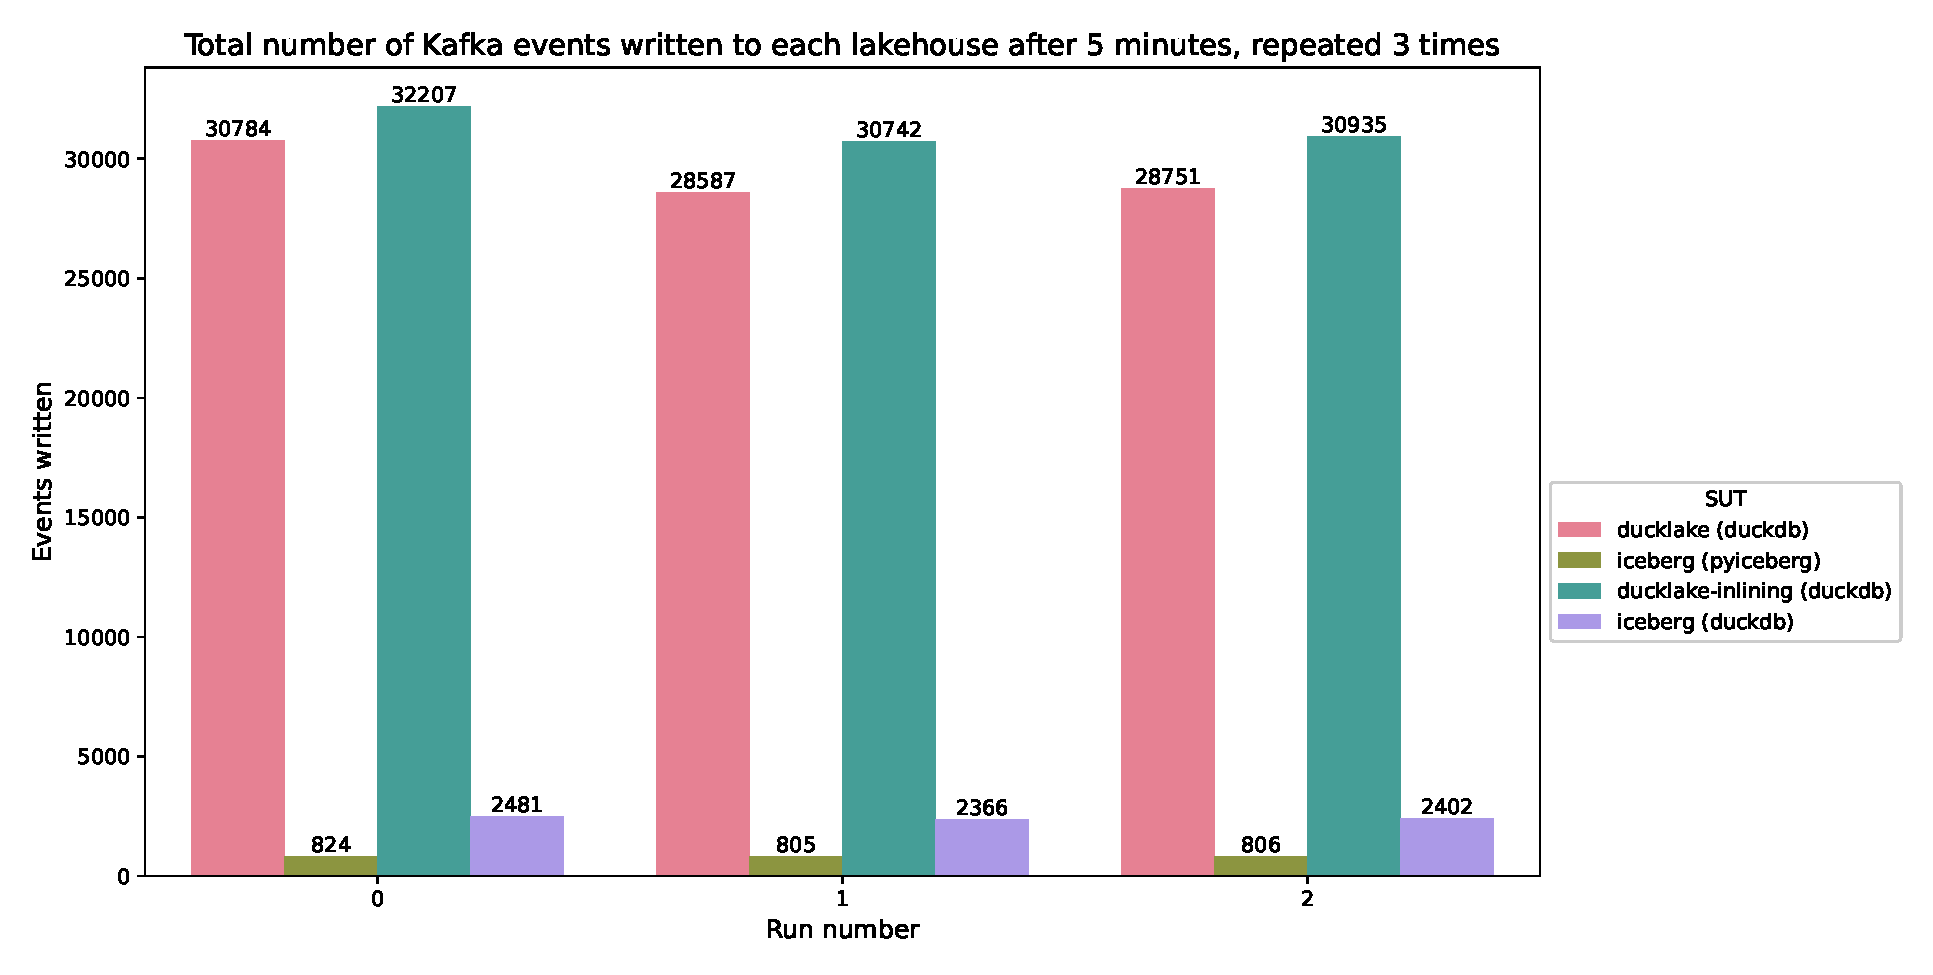
\includegraphics[width=\linewidth]{imgs/total-individual-events-written.eps}
	\caption{Number of events written one by one to each SUT in a time span of 5 minutes. The run numbers correspond to the repetitions of each experiment, where run 0 is considered cold and runs 1 and 2 are considered warm.}
	\label{fig:total-individual-events-written}
\end{figure}

Looking at the amount of events written to the different SUTs in Figure \ref{fig:total-individual-events-written}, we can see that DuckLake had a much higher throughput than Iceberg. Using DuckDB did improve Iceberg's throughput, but it was nonetheless much lower than DuckLake's.

\begin{figure}[h!]
	\centering
	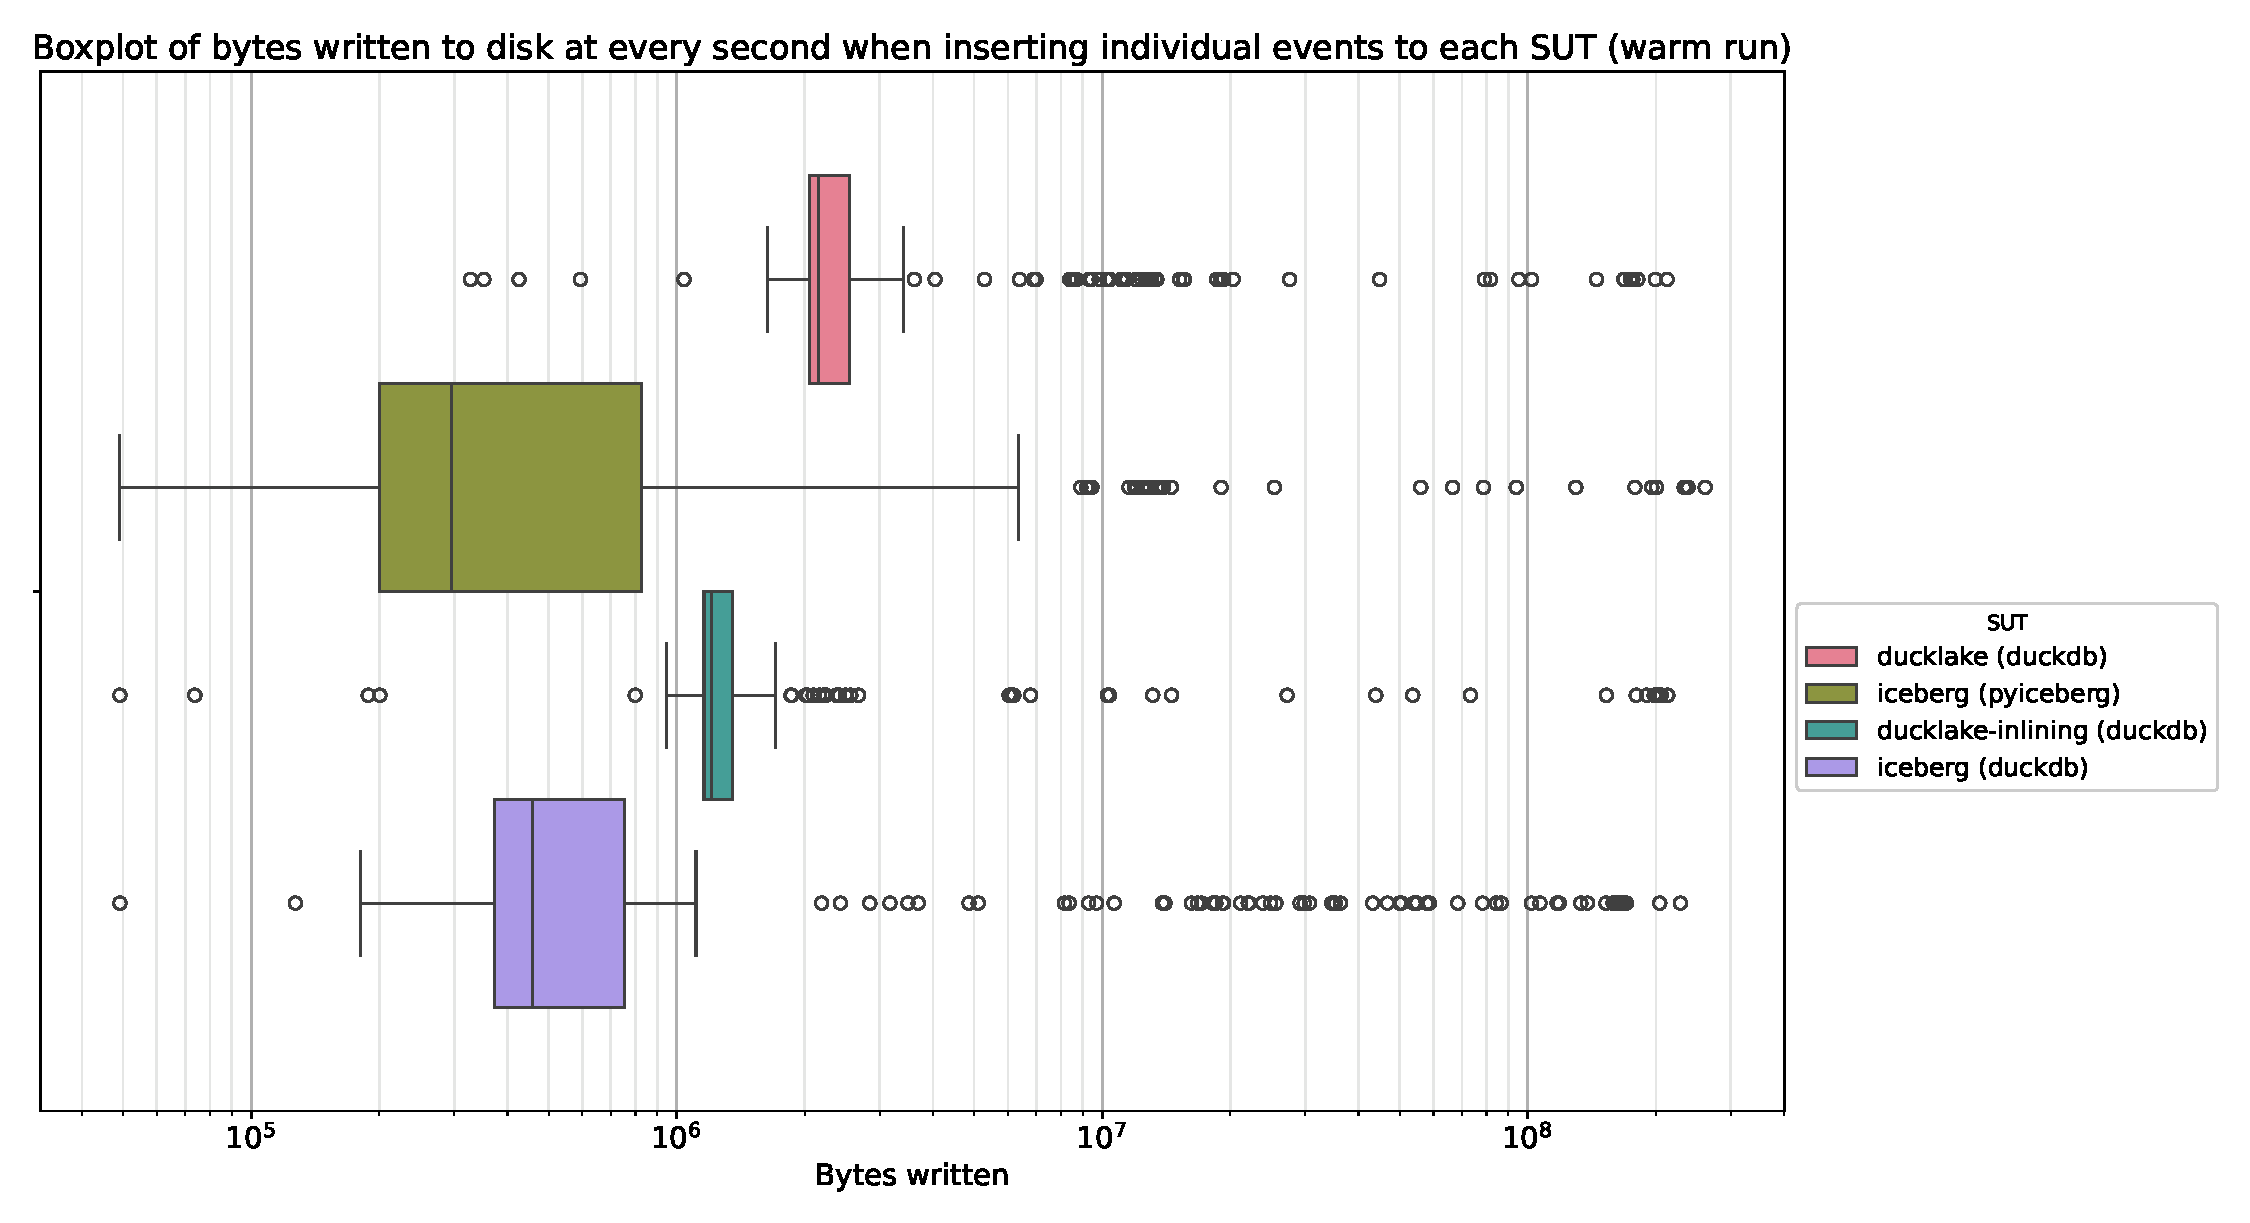
\includegraphics[width=\linewidth]{imgs/box-bytes-written-individual.eps}
	\caption{Boxplot of bytes written to disk at every second when inserting individual events to each SUT (warm run). The measurements were taken at intervals of 1 second.}
	\label{fig:box-bytes-written-individual}
\end{figure}

\begin{table}[h!]
	\centering
	\begin{tabular}{|c|c|c|}
		\hline
		\textbf{SUT} & \textbf{Median (MB)} & \textbf{IQR (MB)} \\
		\hline
		DuckLake & 2.154 & 0.502 \\
		\hline
		Iceberg (PyIceberg) & 0.291 & 0.594 \\
		\hline
		DuckLake + Inlining & 1.204 & 0.193 \\
		\hline
		Iceberg (DuckDB) & 0.459 & 0.380 \\
		\hline
	\end{tabular}
	\caption{Median and interquartile range, in megabytes, of the box plots presented in Figure \ref{fig:box-bytes-written-individual}.}
	\label{tab:median-iqr-box-bytes-individual}
\end{table}

Focusing now on the first warm run of each SUT, we see from Figure \ref{fig:box-bytes-written-individual} that DuckLake was often able to write more bytes per second than Iceberg, which is in line with the total events written, shown in Figure \ref{fig:total-individual-events-written}. We can also see from Table \ref{tab:median-iqr-box-bytes-individual} that the median number of bytes written to DuckLake was about an order of magnitude larger than that of Iceberg with PyIceberg. In addition, Iceberg + PyIceberg seems to have a more unstable rate of bytes/second, which is reflected by the highest interquartile range, i.e. spread, presented in Table \ref{tab:median-iqr-box-bytes-individual}.

\subsection{Write times}
Looking at Figure \ref{fig:box-write-times-individual}, we can see that DuckLake has more consistent write times than Iceberg + PyIceberg, based on the difference in the spread between them. Using Iceberg with DuckDB produces a smaller spread, and thus more consistent write times, but its median is still around an order of magnitude slower than both DuckLake runs. The median write times of each SUT are consistent with their respective amount of bytes/second and events written (Figures \ref{fig:box-bytes-written-individual} and \ref{fig:total-individual-events-written}).

\begin{figure}[h!]
	\centering
	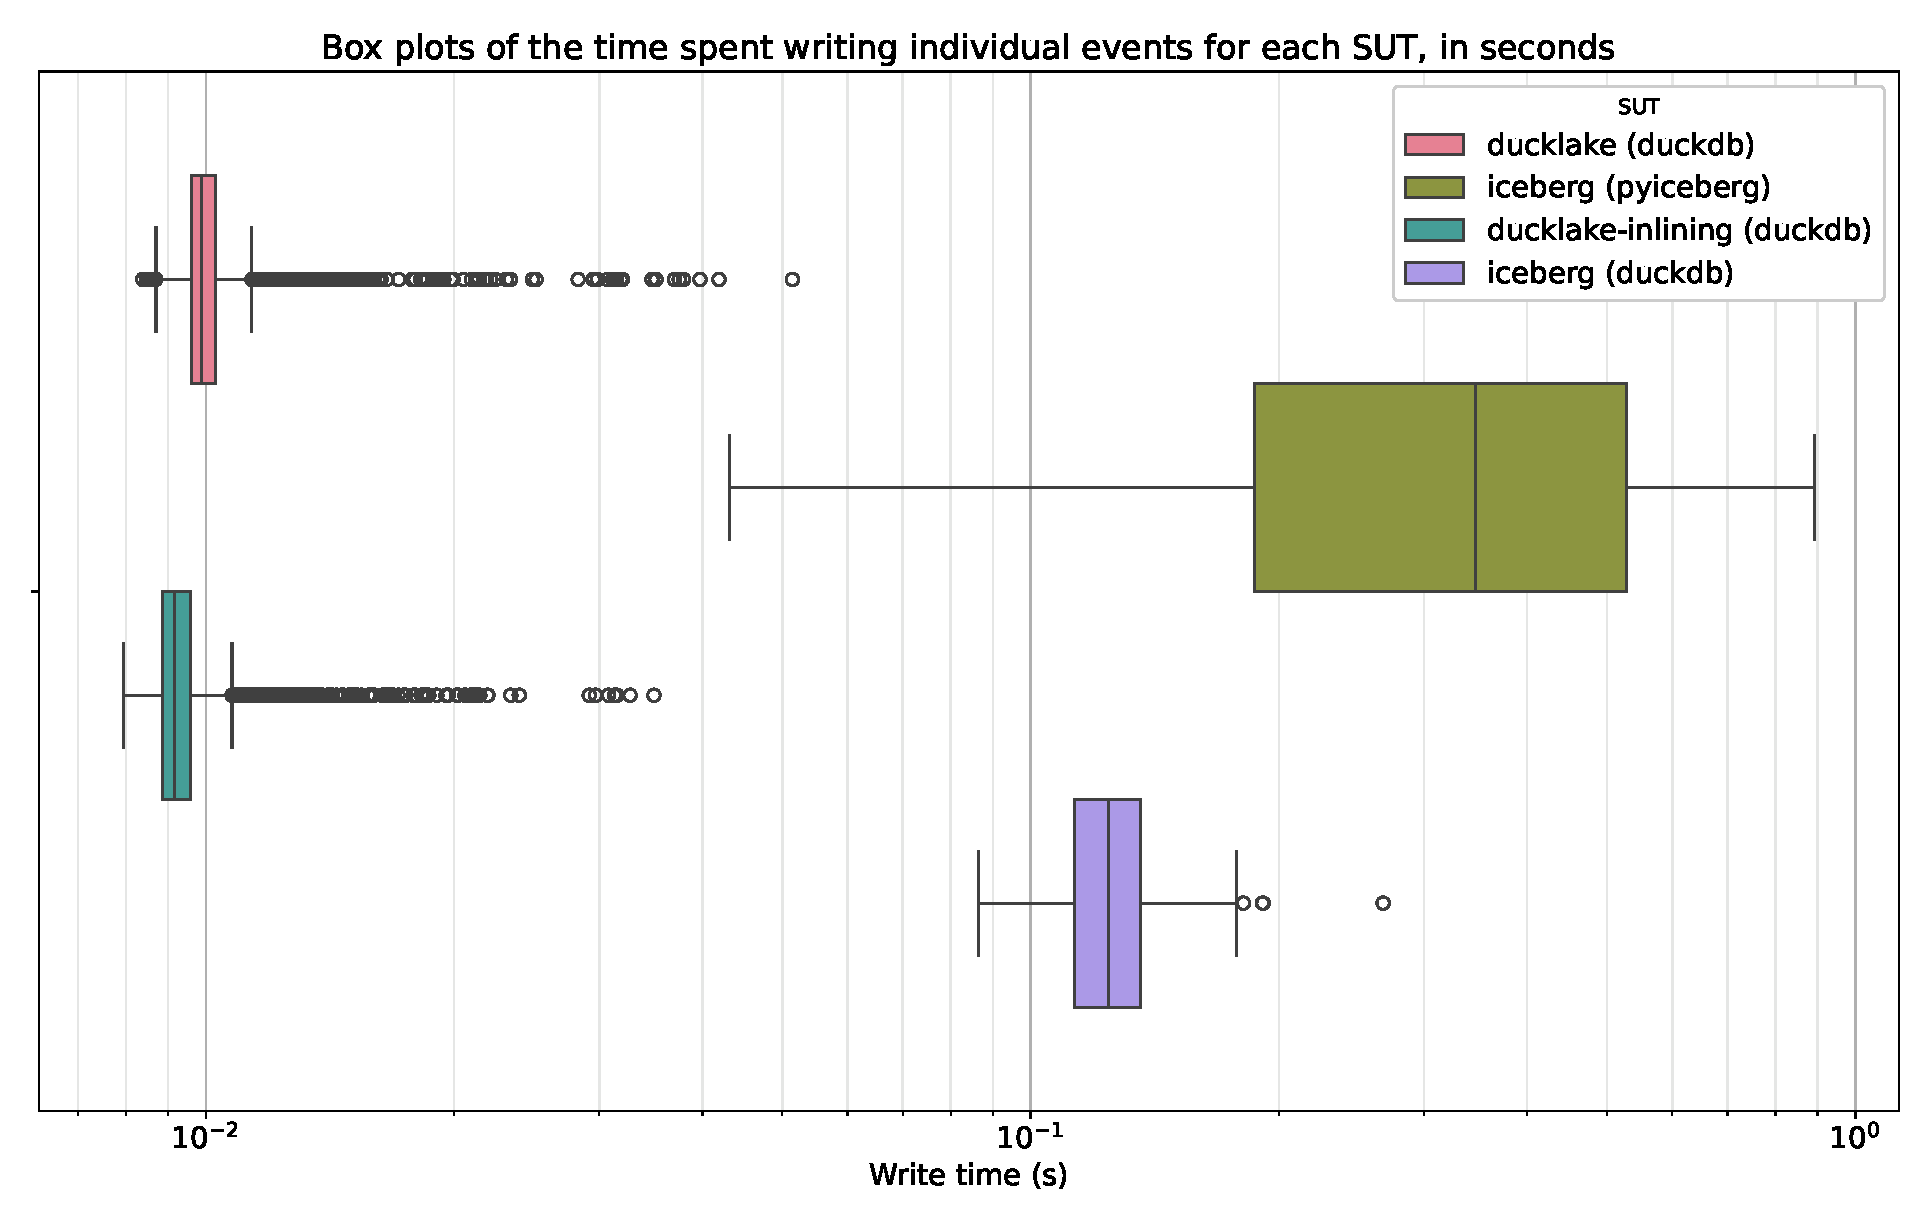
\includegraphics[width=\linewidth]{imgs/box-write-times-individual.eps}
	\caption{Box plots of the time spent writing each individual event to the lakehouse tables during the first warm run, in seconds.}
	\label{fig:box-write-times-individual}
\end{figure}

\begin{table}[h!]
	\centering
	\begin{tabular}{|c|c|c|}
		\hline
		\textbf{SUT} & \textbf{Median (ms)} & \textbf{IQR (ms)} \\
		\hline
		DuckLake & 9.889 & 0.667 \\
		\hline
		Iceberg (PyIceberg) & 346.208 & 341.194 \\
		\hline
		DuckLake + Inlining & 9.169 & 0.711 \\
		\hline
		Iceberg (DuckDB) & 124.303 & 22.650 \\
		\hline
	\end{tabular}
	\caption{Median and interquartile range, in milliseconds, of the box plots presented in Figure \ref{fig:box-write-times-individual}.}
	\label{tab:median-iqr-box-write-times-individual}
\end{table}

We observed that the write times for Iceberg increase over time, as shown in Figure \ref{fig:scatter-write-times-over-time-individual}, which explains the larger spread in the data when compared to other SUTs. Although using Iceberg with DuckDB help control the spread of write times, we can see from Figure \ref{fig:scatter-write-times-over-time-individual} that they still get larger, as more data is written. By contrast, DuckLake's write times seems to stay more or less constant throughout the whole run.

\begin{figure}[h!]
	\centering
	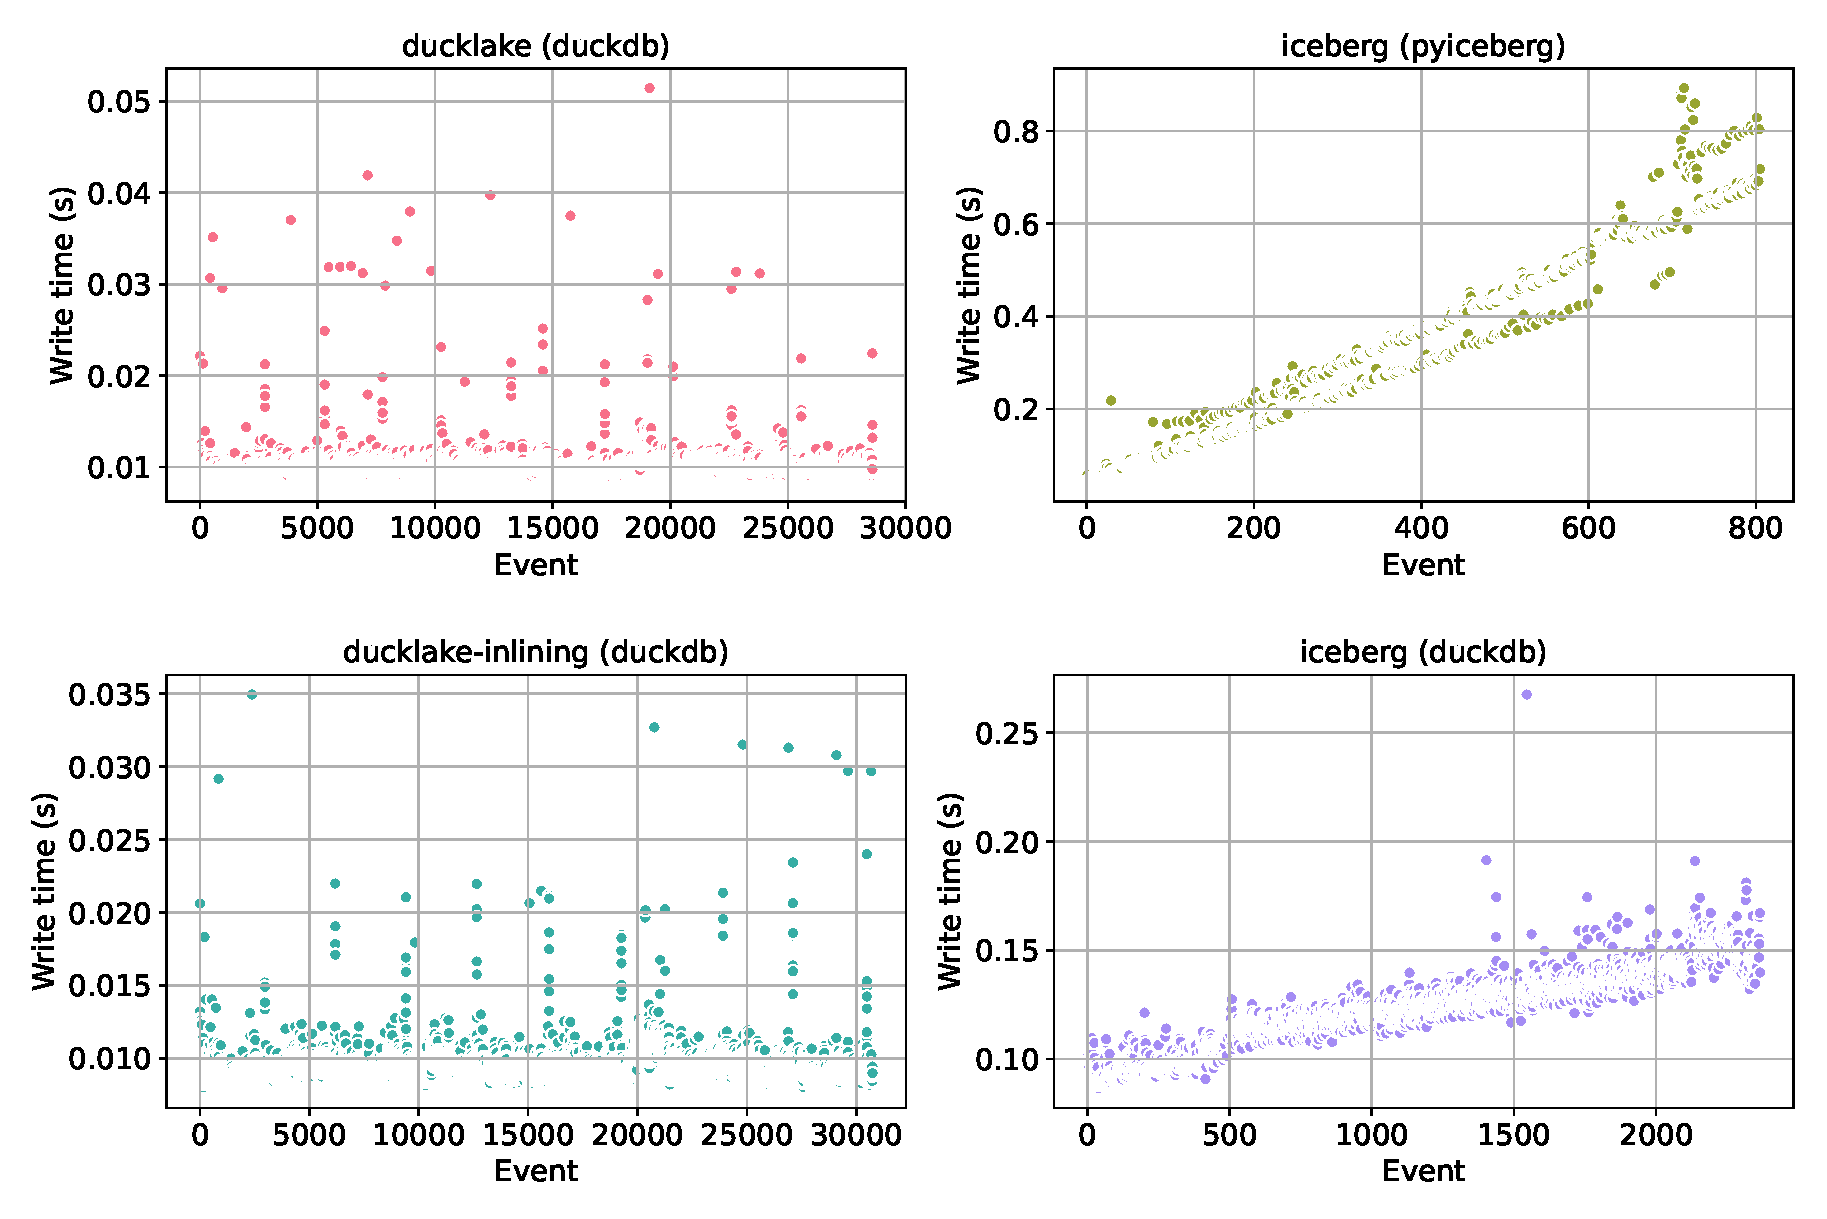
\includegraphics[width=\linewidth]{imgs/scatter-write-times-over-time-individual.eps}
	\caption{Scatter plot of time spent writing individual event to the lakehouse tables during the first warm run, in seconds.}
	\label{fig:scatter-write-times-over-time-individual}
\end{figure}


\begin{table}[h!]
	\centering
	\begin{tabular}{|c|c|}
		\hline
		\textbf{Run number} & \textbf{Flush time (ms)} \\
		\hline
		0 & 219.874 \\
		\hline
		1 & 205.867 \\
		\hline
		2 & 193.615 \\
		\hline
	\end{tabular}
	\caption{Time taken by each DuckLake + Inlining run to flush inlined data to a single Parquet file, in milliseconds.}
	\label{tab:times-flush-inlined-individual}
\end{table}

Regarding the DuckLake instance with inlining enabled, we find that the time taken to flush the inlined events to a Parquet file on disk was around 200 milliseconds, as shown in Table \ref{tab:times-flush-inlined-individual}. This is about $20\times$ slower than the median write time of DuckLake without inlining, and about $2\times$ slower than the median of Iceberg with DuckDB. However, DuckLake with inlining enabled was able to outperform the median write time of Iceberg with PyIceberg by around $1.5\times$.

\subsection{Read times}

\begin{figure}[h!]
	\centering
	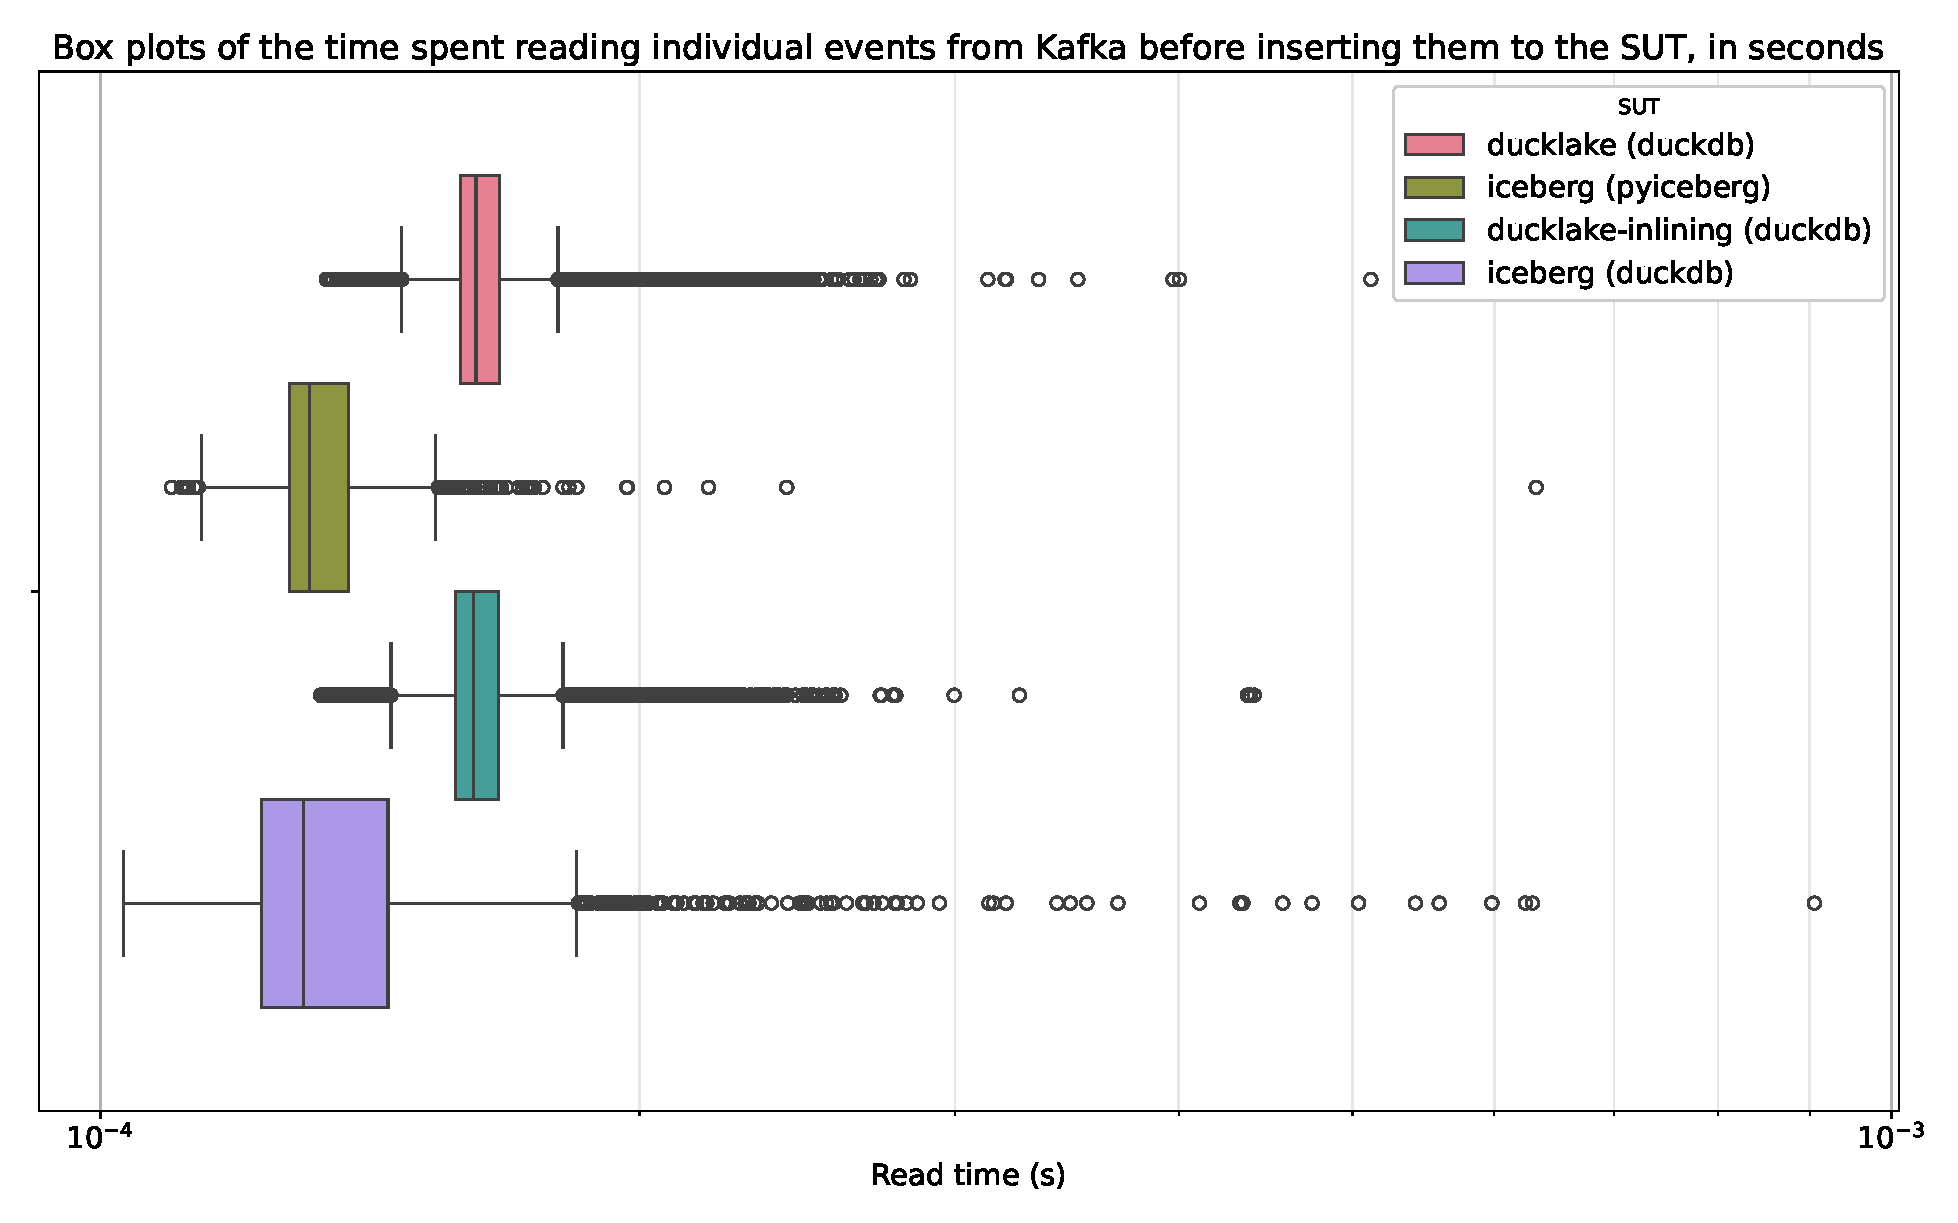
\includegraphics[width=\linewidth]{imgs/box-read-times-individual.eps}
	\caption{Box plots of the time spent reading individual events from Kafka during the first warm run of each SUT, in seconds.}
	\label{fig:box-read-times-individual}
\end{figure}

The box plots in Figure \ref{fig:box-read-times-individual} go over the time spent reading each individual event from the Kafka broker. We can see that the median read times of DuckLake runs were slightly higher than Iceberg's, but the almost all read times were lower than 1 millisecond, with most times staying between 0.1 and 0.2 milliseconds. These measurements indicate that no system had a major advantage over others due to significantly higher read times.

\subsection{CPU usage}
We observed that Iceberg with DuckDB consistently utilized a higher percentage of the CPU than the other three SUTs. Nonetheless, all systems were mostly stable throughout the runs, except for a few spikes and dips, as shown in Figure \ref{fig:cpu-usage-individual-events}. These observations can be attributed to the noise caused by other processes running in the background, such as the Docker containers or even OS processes.

\begin{figure}[h!]
	\centering
	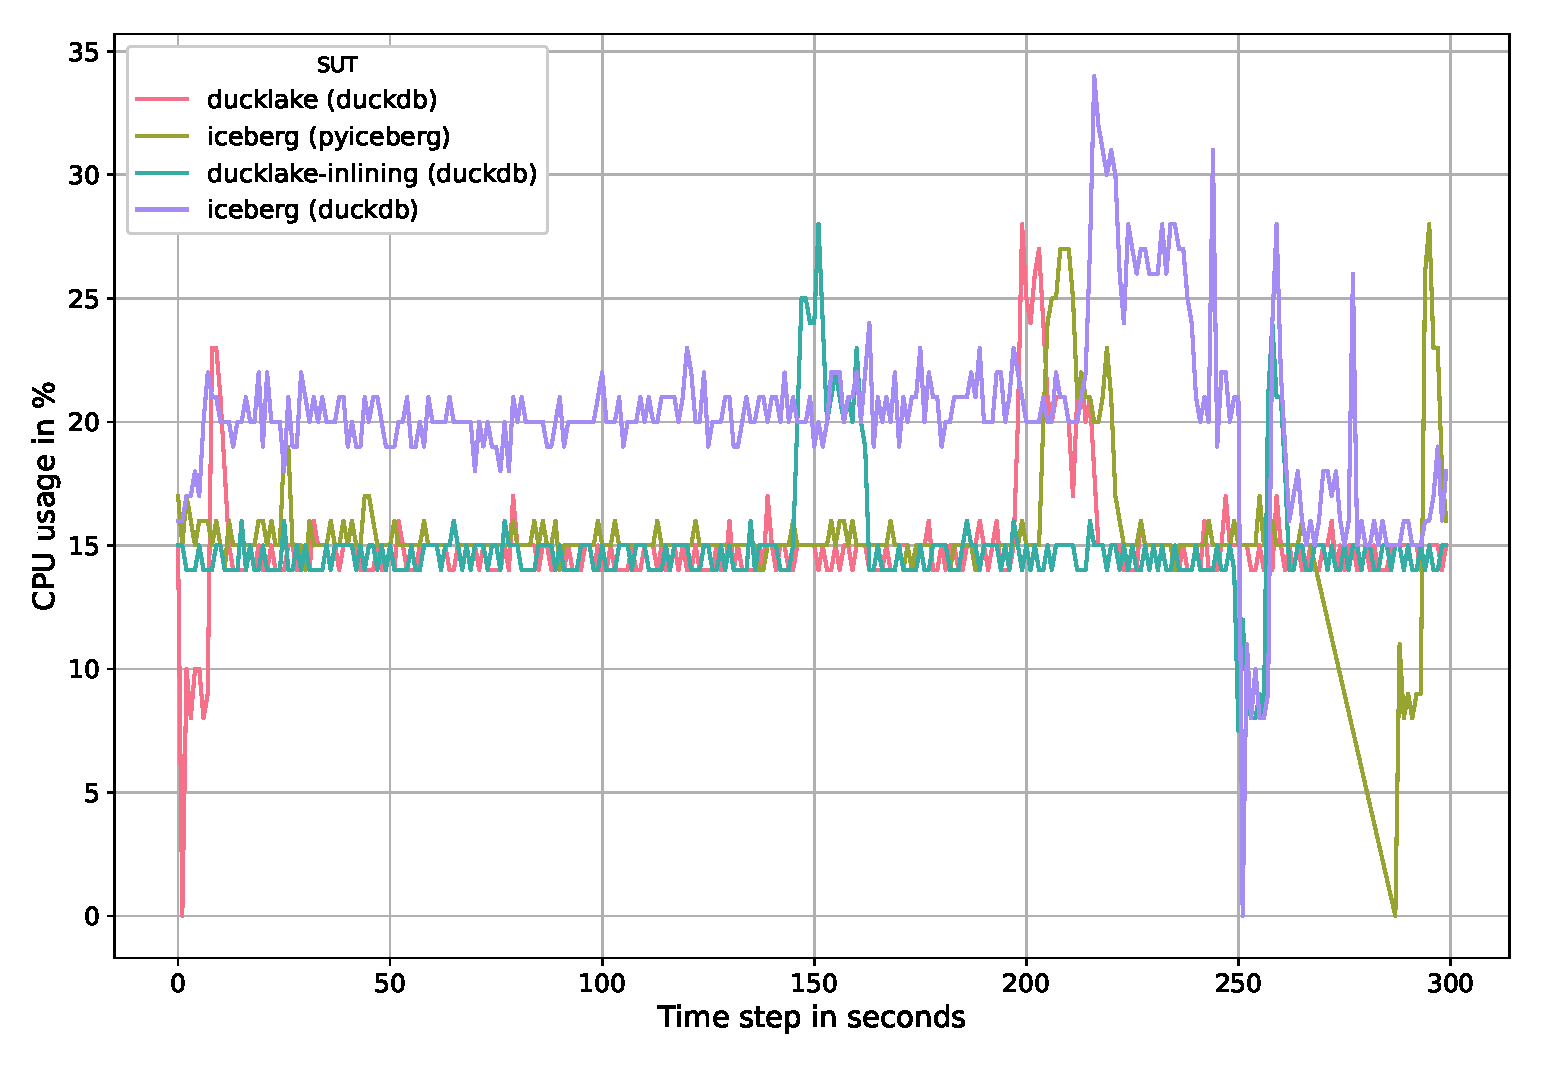
\includegraphics[width=\linewidth]{imgs/cpu-usage-individual-events.eps}
	\caption{CPU usage percentage measured at every second throughout each run of writing individual events to SUTs.}
	\label{fig:cpu-usage-individual-events}
\end{figure}

\section{Writing events in batches of 1,000}

\subsection{Total events written}
Figure \ref{fig:total-batched-events-written} shows the total number of events written to each SUT when writing data in batches of 1,000 events. As observed in the previous experiments, the cold run was slightly better than the warm runs, so we focus on the latter instead.

We can see that all systems performed significantly better than when events were written one by one to the lakehouse tables. The biggest improvement can be noticed when using Iceberg with DuckDB, which managed to surpass DuckLake with inlining enabled. We also observed that inlining led to a decrease of  in the amount of events written to DuckLake. That is in contrast to the previous experiments, where inlining had in fact improved the throughput of DuckLake.

\begin{figure}[h!]
	\centering
	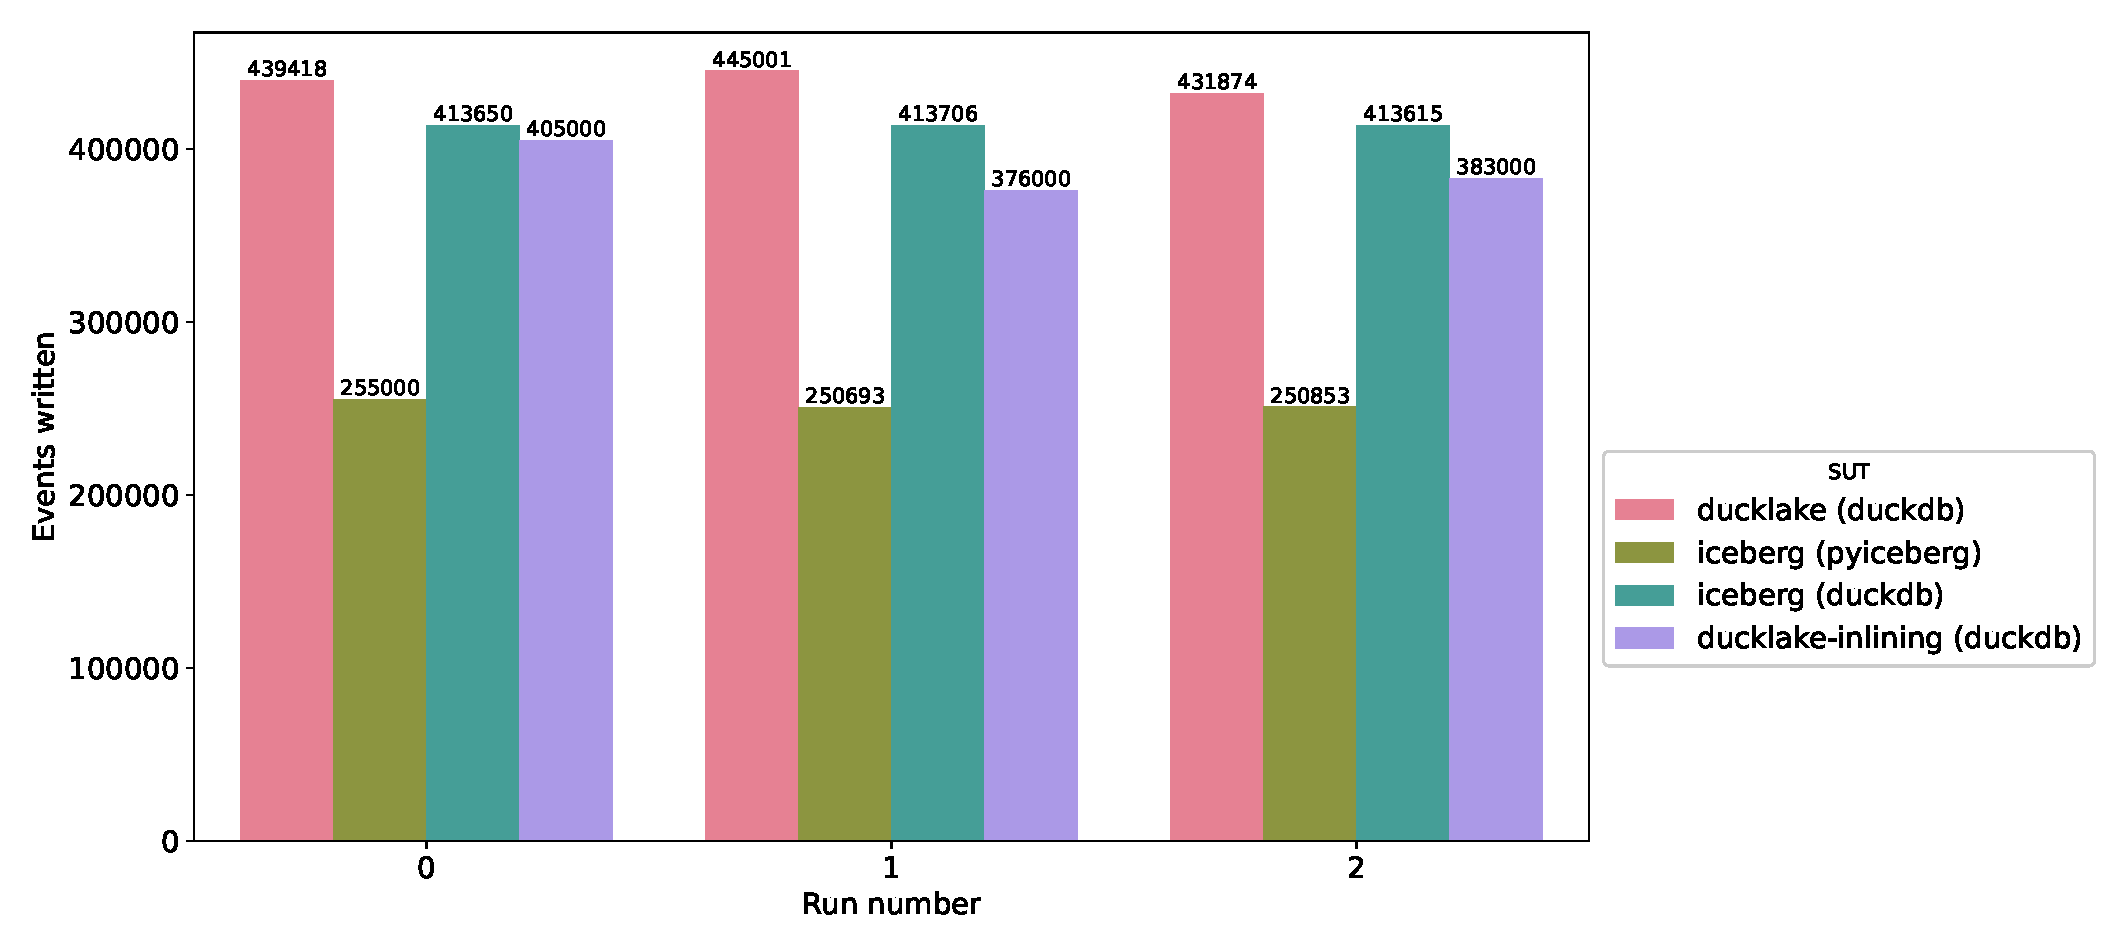
\includegraphics[width=\linewidth]{imgs/total-batched-events-written.eps}
	\caption{Number of events written in batches of 1,000 to each SUT in a time span of 5 minutes. The run numbers correspond to the repetitions of each experiment, where run 0 is considered cold and runs 1 and 2 are considered warm.}
	\label{fig:total-batched-events-written}
\end{figure}

When looking at the amount of bytes written at every second in Figure \ref{fig:box-bytes-written-batched}, we see that all systems wrote fewer bytes per second than when writing events one by one. From Table \ref{tab:median-iqr-box-bytes-batched} we can see that median number of bytes written to disk differed less between the SUTs than in the previous experiment. The exception here was DuckLake + inlining, which had a median about twice as big as the second highest median.

In terms of the spread of the data, both DuckLake instances wrote bytes at a more consistent rate than the Iceberg instances. In contrast to the previous experiment, DuckDB worsened Iceberg's data spread when compared to PyIceberg. In addition, DuckLake with inlining and Iceberg + DuckDB had less stable rates of bytes/second than their counterparts in the previous experiment. Overall, Iceberg + PyIceberg differed the least between writing individual and batched events, whereas all other three SUTs had a lower median number of bytes written per second.

\begin{figure}[h!]
	\centering
	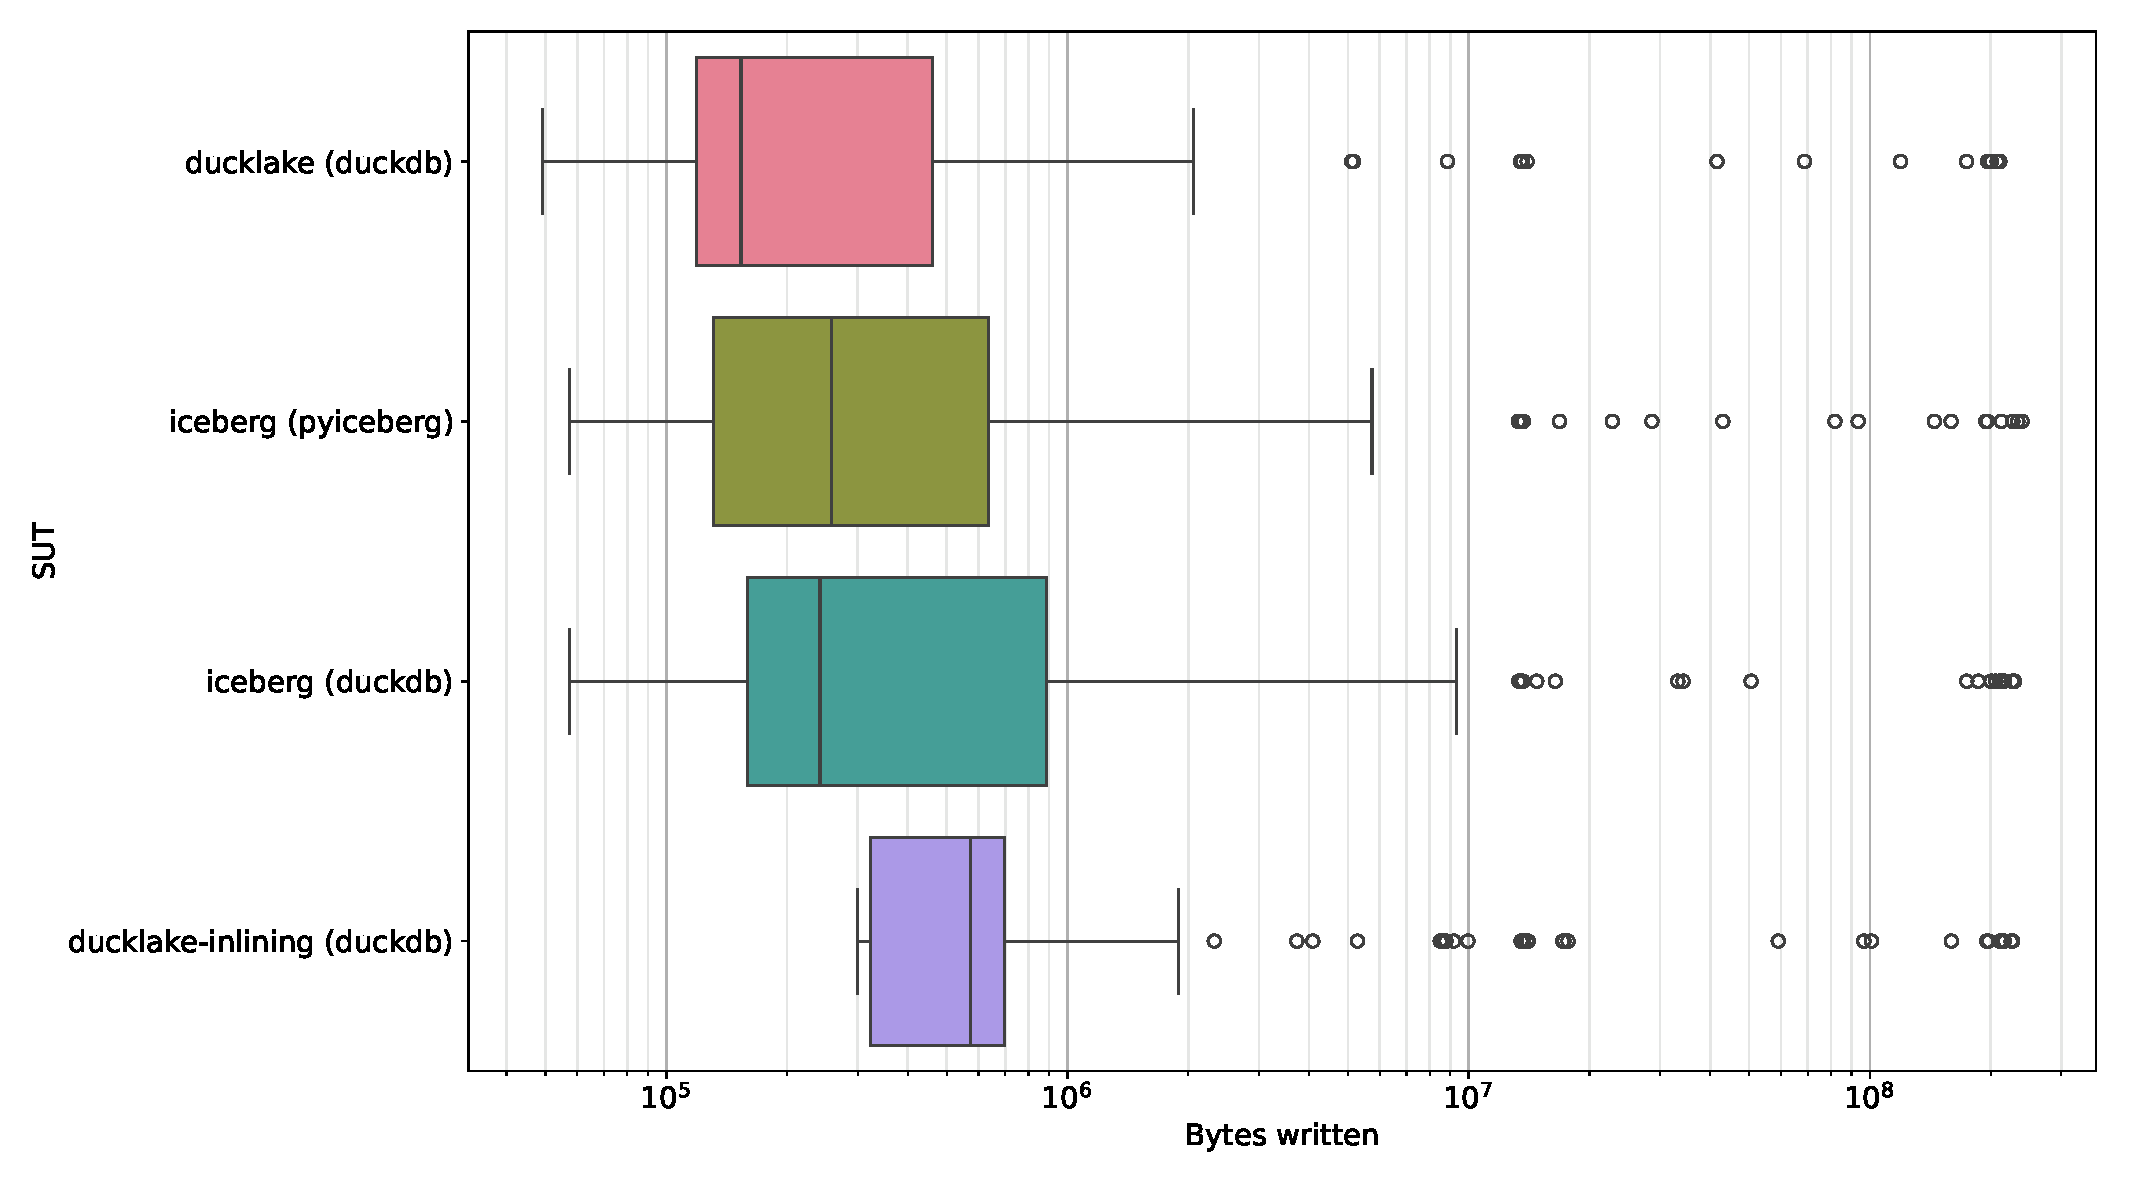
\includegraphics[width=\linewidth]{imgs/box-bytes-written-batched.eps}
	\caption{Boxplot of bytes written to disk at every second when inserting individual events to each SUT (warm run). The measurements were taken at intervals of 1 second.}
	\label{fig:box-bytes-written-batched}
\end{figure}

\begin{table}[h!]
	\centering
	\begin{tabular}{|c|c|c|}
		\hline
		\textbf{SUT} & \textbf{Median (MB)} & \textbf{IQR (MB)} \\
		\hline
		DuckLake & 0.154 & 0.341 \\
		\hline
		Iceberg (PyIceberg) & 0.258 & 0.502 \\
		\hline
		Iceberg (DuckDB) & 0.242 & 0.727 \\
		\hline
		DuckLake + Inlining & 0.573 & 0.372 \\
		\hline
	\end{tabular}
	\caption{Median and interquartile range, in megabytes, of the box plots presented in Figure \ref{fig:box-bytes-written-batched}.}
	\label{tab:median-iqr-box-bytes-batched}
\end{table}


\subsection{Write times}
The write times of the SUTs shown in Figure \ref{fig:box-write-times-batched} are in line with the results presented in Figure \ref{fig:total-batched-events-written}. We see that Iceberg + PyIceberg had the highest write times of all SUTs, with a median write time about $3\times$ higher than the second highest median (DuckLake + Inlining). For all SUTs the median write time was higher than the previous experiments because every write operation involved batches of 1,000 event, in contrast to individual events in the previous experiment.

Regarding stability of write times, Iceberg + PyIceberg was also least stable system, given by its higher IQR. All the three other systems showed a similar, lower spread in their write times.

With respect to the flush times of DuckLake + inlining, we see in Table \ref{tab:times-flush-inlined-batched} that it took around 2 seconds to flush the inlined data. This represents a tenfold increase compared to the previous experiment. Furthermore, the flush times were about $3\times$ slower than the highest median write time.

\begin{figure}[h!]
	\centering
	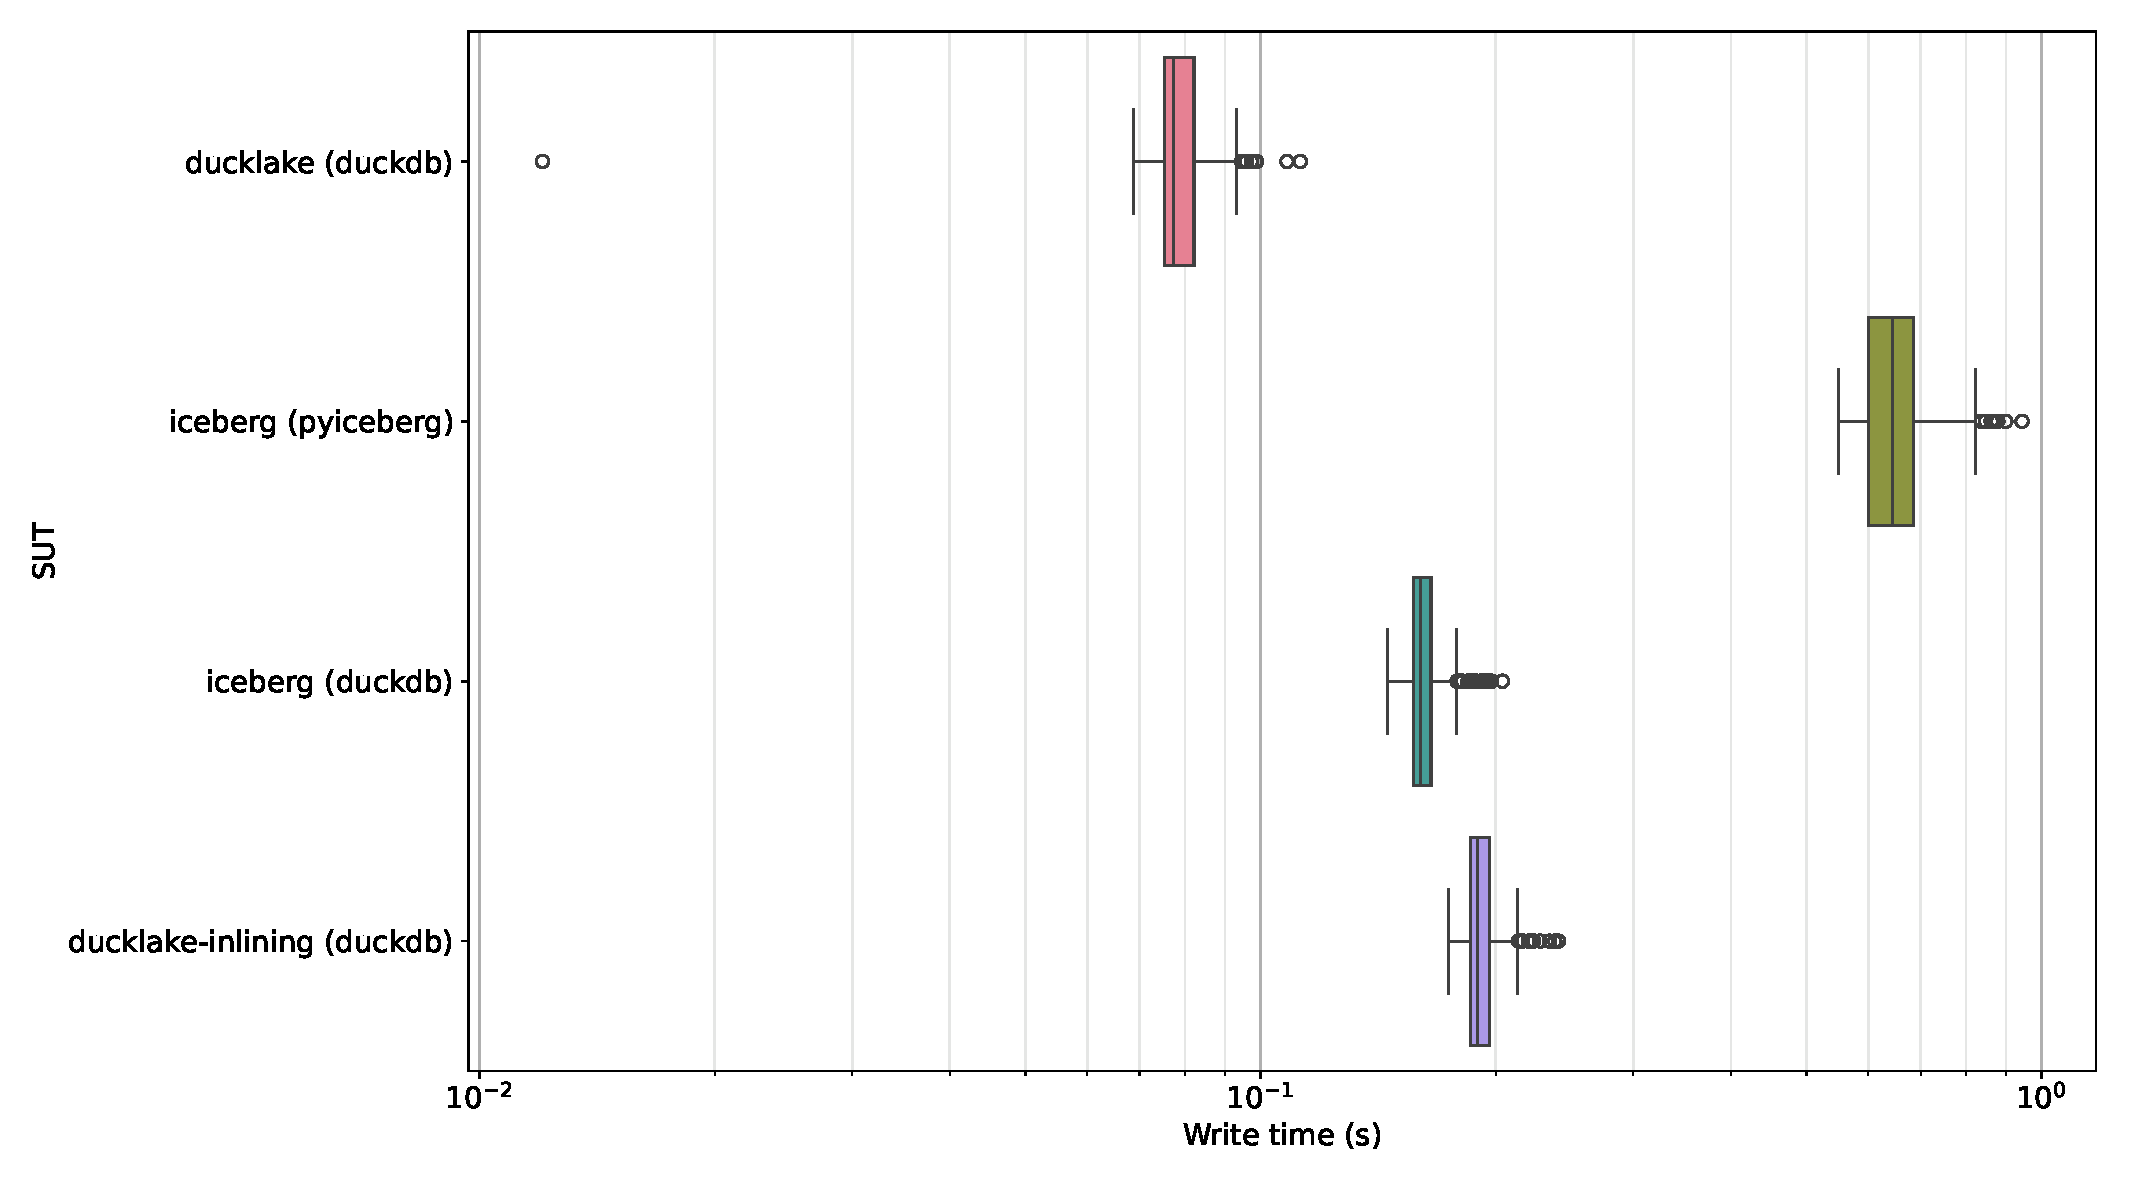
\includegraphics[width=\linewidth]{imgs/box-write-times-batched.eps}
	\caption{Box plots of the time spent writing each batch of 1,000 events to the lakehouse tables during the first warm run, in seconds.}
	\label{fig:box-write-times-batched}
\end{figure}

\begin{table}[h!]
	\centering
	\begin{tabular}{|c|c|c|}
		\hline
		\textbf{SUT} & \textbf{Median (ms)} & \textbf{IQR (ms)} \\
		\hline
		DuckLake & 77.439 & 6.942 \\
		\hline
		Iceberg (PyIceberg) & 644.842 & 84.695 \\
		\hline
		DuckLake + Inlining & 189.746 & 10.625 \\
		\hline
		Iceberg (DuckDB) & 160.086 & 8.189 \\
		\hline
	\end{tabular}
	\caption{Median and interquartile range, in milliseconds, of the box plots presented in Figure \ref{fig:box-write-times-batched}.}
	\label{tab:median-iqr-box-write-times-batched}
\end{table}

\begin{table}[h!]
	\centering
	\begin{tabular}{|c|c|}
		\hline
		\textbf{Run number} & \textbf{Flush time (s)} \\
		\hline
		0 & 2.287 \\
		\hline
		1 & 1.992 \\
		\hline
		2 & 1.974 \\
		\hline
	\end{tabular}
	\caption{Time taken by each DuckLake + inlining run to flush the inlined batches of data to a single Parquet file, in seconds.}
	\label{tab:times-flush-inlined-batched}
\end{table}

Looking now at Figure \ref{fig:scatter-write-times-over-time-batched}, we can see that write times behave in a similar way as the previous experiment. When using Iceberg with PyIceberg, we see the same effect where write times get larger as more events are added to the Iceberg table, which again explains the bigger spread of Iceberg's write times presented in Table \ref{tab:median-iqr-box-write-times-batched}. DuckLake + DuckDB had the lowest and more consistent write times, with the other two SUTs presenting occasional spikes in write times, but staying mostly consistent throughout the experiment run.

\begin{figure}[h!]
	\centering
	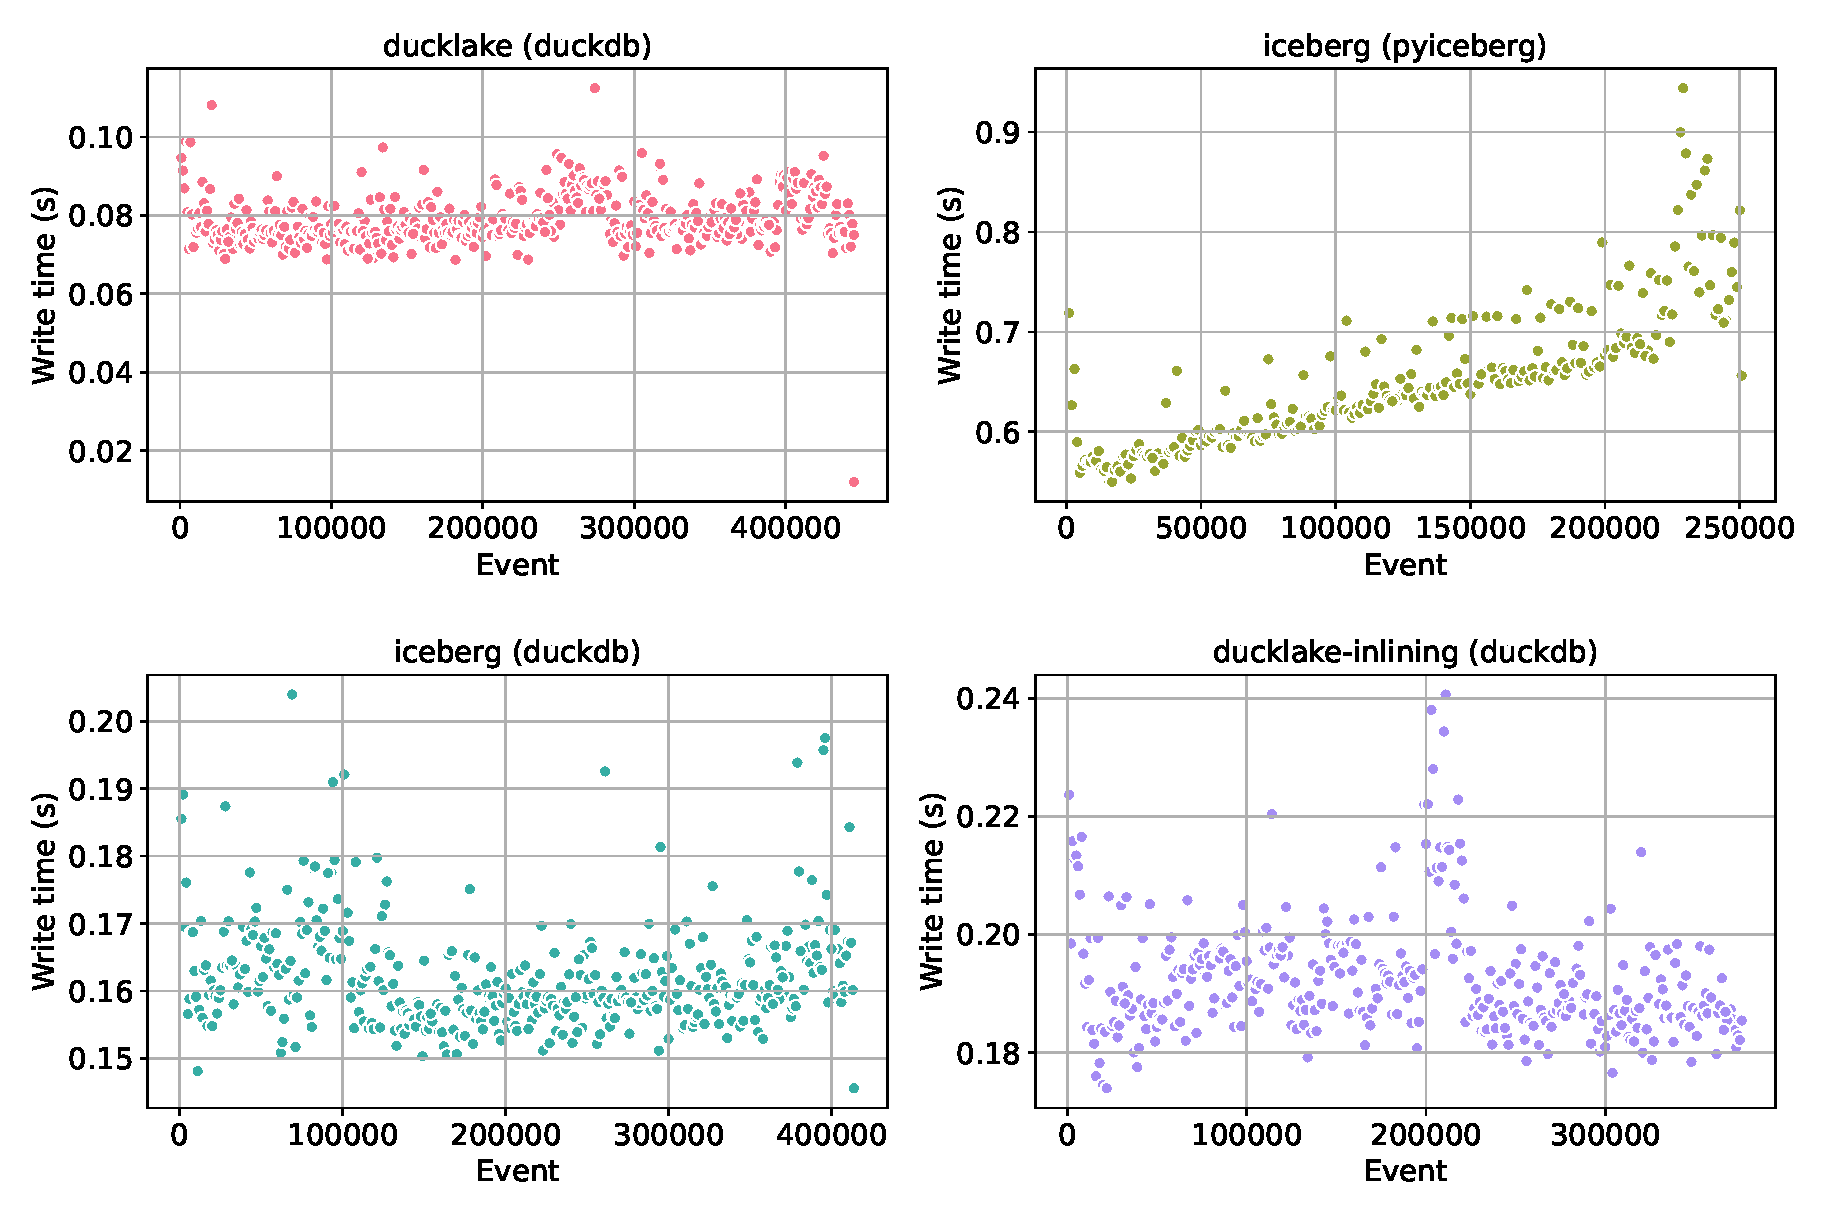
\includegraphics[width=\linewidth]{imgs/scatter-write-times-over-time-batched.eps}
	\caption{Scatter plot of time spent writing batches of 1,000 events to the lakehouse tables during the first warm run, in seconds.}
	\label{fig:scatter-write-times-over-time-batched}
\end{figure}

\subsection{Read times}
The read times of all runs (Figure \ref{fig:box-read-times-batched}) were very similar to each other, with the Q3 for all box plots being below 0.1 milliseconds. We can again confirm that no SUT had an unfair advantage caused by significantly faster read times of our benchmark tool.

\begin{figure}[h!]
	\centering
	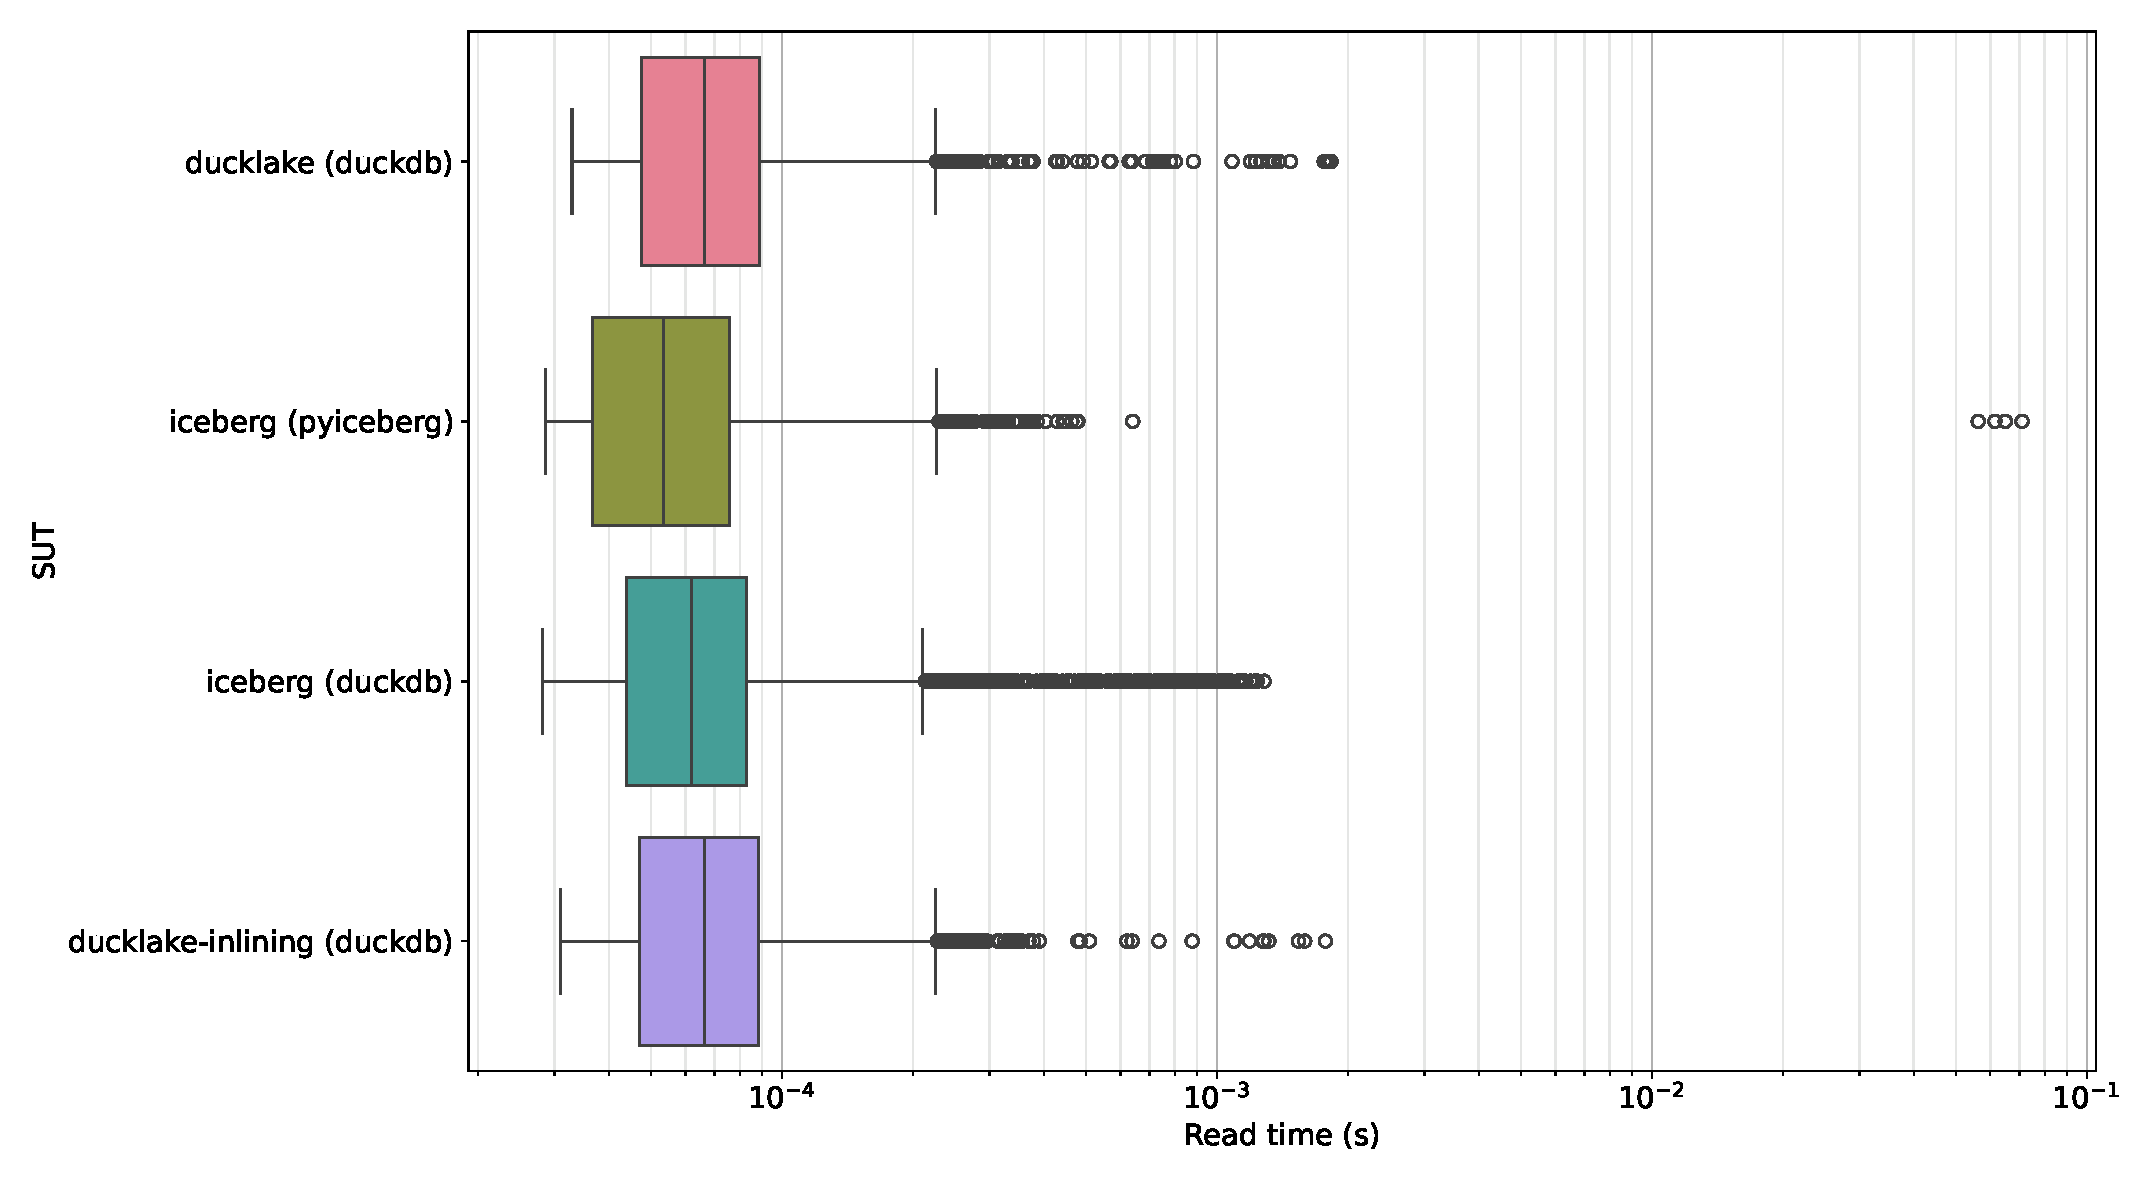
\includegraphics[width=\linewidth]{imgs/box-read-times-batched.eps}
	\caption{Box plots of the time spent reading individual events from Kafka during the first warm run of each SUT, in seconds.}
	\label{fig:box-read-times-batched}
\end{figure}

\subsection{CPU usage}
In terms of CPU usage, all systems presented very similar percentages throughout their runs, as we can see in Figure \ref{fig:cpu-usage-batched-events}. DuckLake instances showed slightly higher CPU percentages overall than Iceberg. We also see that all four runs had a dip and spike around halfway through, which is likely due to some underlying operation running in the local machine's OS.

\begin{figure}[h!]
	\centering
	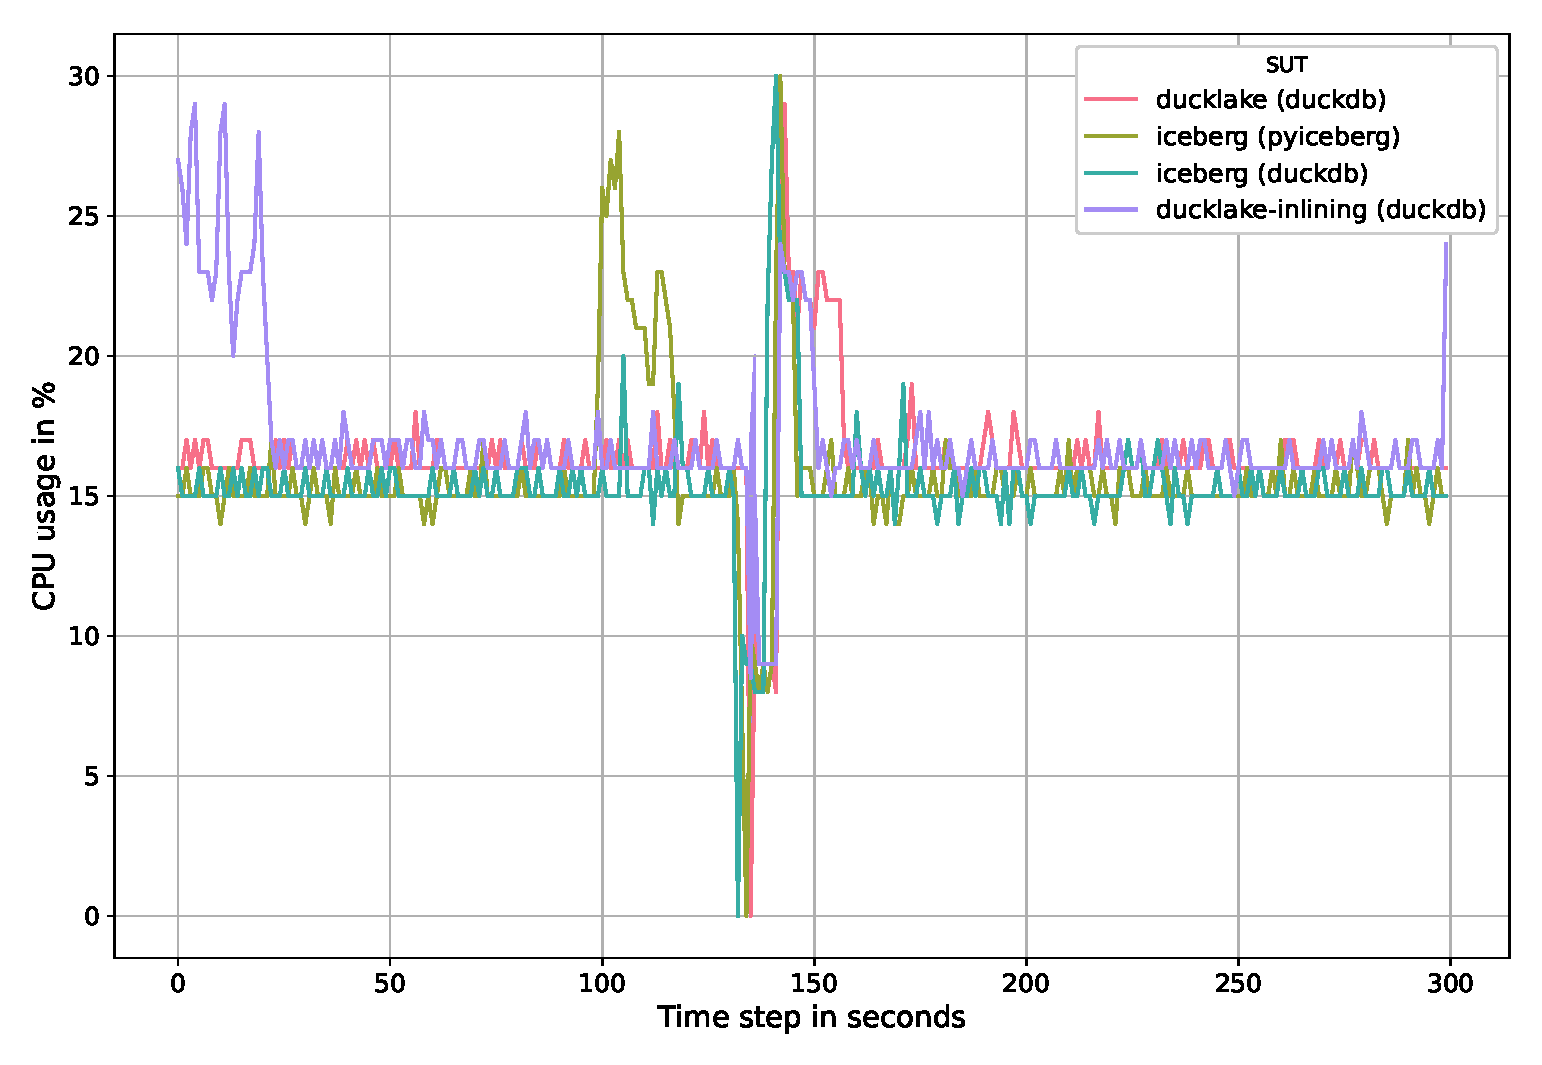
\includegraphics[width=\linewidth]{imgs/cpu-usage-batched-events.eps}
	\caption{Time spent reading individual events from Kafka during the first warm run of each SUT. The measurements were taken using time.perf\_counter\_ns.}
	\label{fig:cpu-usage-batched-events}
\end{figure}



\chapter{Discussion}\label{ch:discussion}

% TODO: Mention that parquet files produced by PyIceberg were significantly bigger than DuckDB (8.2 kB vs 2.9 kB), even though both use snappy compression.

\section{DuckDB vs. PyIceberg}
We would first like to discuss the differences observed between DuckDB and PyIceberg, when running experiments with Iceberg. The difference in throughput between the two clients was considerably large when writing both individual events and batches of events.

\subsection{Faster write operations}
If we look at the experiments where events were written one by one to the Iceberg table, we see that Parquet files written by DuckDB are 2.9 kB in size, while PyIceberg produced files of 8.2 kB. This difference of almost $3\times$ in size is surprising, given that both clients were configured to use snappy compression (Section \ref{sec:configuration}). We believe this difference might be caused by PyIceberg not applying compression to files that contain few rows. Our reason for this claim is that when writing batches of 1,000 events, both DuckDB and PyIceberg produced Parquet files of similar size, ranging between 37 kB and 40 kB.

We expect similar internal differences to be present in the implementation of DuckDB's and PyIceberg's JSON and Avro writers as well. For instance, Iceberg's metadata JSON files will grow larger with time because they contain all the data from previous metadata files. As a consequence, write times will increase after each append, as we observed in Figure \ref{fig:scatter-write-times-over-time-individual}. However, the write times of DuckDB increased at a much slower rate than PyIceberg's did. We believe this difference is thus linked to a more efficient implementation of DuckDB's metadata writer. This would also explain why DuckDB was still faster than PyIceberg when writing batches of 1,000 events, given that the Parquet file sizes were similar between both clients in that case.

Considering these differences between DuckDB and PyIceberg, we focus our discussion on the results on PyIceberg + DuckDB, unless explicitly said otherwise.

\section{Single events vs. batches}

\subsection{Throughput}
Writing events in batches significantly improved the throughput of all systems. This is also reflected by the increase in the median write time relative to the increase in events written per file. While we increased the latter by a factor of 1,000$\times$, the former increased by $20\times$ at most (DuckLake + Inlining). This performance increase is directly tied to how Parquet files work: The file format is meant for efficiently storing compressed columnar data in row groups, so that it can be used for analytics tasks \cite{ParquetMotivation2022}. It also stores metadata to further improve read efficiency. Consequently, the overhead associated with writing a Parquet file makes it more well suited for multiple rows (events) per file, rather than a single row. In fact, the recommended row group size is between 512 MB and 1 GB \cite{ParquetConfigurations2024}.

Despite the performance gains brought by writing data in batches, we would like to stress the significant differences between Iceberg and DuckLake when writing individual events. The results presented in Figure \ref{fig:total-individual-events-written} highlight the impact of each system's design on their throughput: Every insert operation in Iceberg will create four files (one data file, one manifest file, one manifest list and one metadata file), and a catalog transaction, that all need to be written sequentially. In addition, the metadata file will become larger each time, thus causing longer write times after each insert (Figure \ref{fig:scatter-write-times-over-time-individual}). By contrast, writing in DuckLake involves writing a Parquet file and performing a transaction to the catalog server. This difference in the design of each system leads to a throughput that is about $12\times$ higher (Figure \ref{fig:total-individual-events-written}).

\subsection{Total bytes written}
When comparing Tables \ref{tab:median-iqr-box-bytes-individual} and \ref{tab:median-iqr-box-bytes-batched}, we noticed the median for all SUTs was lower when writing batched events than when individual events were written, even though the total number of events was higher in the former setting. This difference can be explained by batched events producing less files overall than individual events. To illustrate this, we looked at the total size of data and metadata files (Avro + JSON) in Iceberg for both settings. When writing individual events to Iceberg, data files accounted for 21.4 MB and metadata files accounted for 5.4 GB. By contrast, when writing batched events, the data files corresponded to 46.4 MB, while metadata files totaled 183.5 MB.

\subsection{Data inlining}
Interestingly, enabling data inlining for DuckLake worsened its performance when writing batched data. In fact, Iceberg was also able to consistently write more events than DuckLake + inlining. This is a surprising result, because inlining does not write any Parquet files, but rather just stores them in the catalog database as part of the transaction. The database still writes that data to disk, which could be slower than writing a Parquet file, thus explaining why inlining becomes slower for a larger amount of data. 

In addition, we saw in Table \ref{tab:median-iqr-box-bytes-batched} that DuckLake with inlining had the highest median number of bytes written to disk. This difference could be explained by the catalog database (PostgreSQL in this case) not compressing the data or compressing it less than the Parquet data. As a consequence, inlining would take more bytes, and thus more time, than directly writing Parquet files for larger batches of data.

It is also worth mentioning that the inlining feature of DuckLake is recommended for small appends/changes by its developers \cite{DuckLakeDocumentationData2025}. So although this feature can be configured for any threshold, it is likely to yield better performance gains for lower amounts of inlined data.

\section{Data inlining trade-off}


\section{Research questions}

\section{Limitations and future work}
Although we did our best to make sure experiments were fair, it is important to acknowledge their limitations. 

Firstly, the experiments were carried out on a single machine, where all services were running in parallel. This means that processes could interfere with each other when trying to acquire system resources, resulting in noise in the data. We believe this is why we observed outliers in our data, especially when looking at CPU usage (Figures \ref{fig:cpu-usage-individual-events} and \ref{fig:cpu-usage-batched-events}) and bytes written per second (Figures \ref{fig:box-bytes-written-individual} and \ref{fig:box-bytes-written-individual}).

Additionally, we believe that running experiments at a larger scale could add more value to our results. Lakehouses usually run in distributed cloud environments, where they are connected to a separate catalog server and storage system. However, running experiments in such an environment brings its own challenges, such as orchestrating multiple cloud services, scaling up services accordingly and accounting for network latency. This would be an interesting challenge to tackle by future work.

Furthermore, our research focused on a scenario where only one client inserts data into the lakehouse tables. However, in many real-life scenarios, data streams are produced by multiple clients, resulting in concurrent insert operations. Evaluating lakehouse systems under those conditions would give more insight into how each of them performs when there are frequent conflicting inserts.
\chapter{Conclusion and future work}\label{ch:conclusion}

\printbibliography

\appendix
\chapter{Additional results}\label{ch:additional-results}

\end{document}
